 % The main file for CAMP reports
 % Don't put any content in here.
%% Draft document mode
%% Final document
\documentclass[11pt,a4paper,bibtotoc,idxtotoc,headsepline,footsepline,footexclude,BCOR14mm,DIV13]{scrbook}

\def\doctype{Bachelor's Thesis in Information Systems}
\def\title{Reinforcement Learning for Adaptive Locomotion of a Snake-like Robot using Tensorflow}
\def\titleGer{Reinforcement Learning zur adaptiven Fortbewegung eines schlangenartigen Roboters mit Tensorflow}
\def\author{Jonathan R\"osner}
\def\date{November 15, 2017}

% text to appear in the footer
\def\footertext{}


% include settings
% Included by MAIN.TEX
% Defines the settings for the CAMP report document

\renewcommand{\sectfont}{\normalfont \bfseries}        % Schriftart der Kopfzeile

% manipulate footer
\usepackage{scrpage2}
\pagestyle{scrheadings}
\ifoot[\footertext]{\footertext} % \footertext set in INFO.TEX
%\setkomafont{pagehead}{\normalfont\rmfamily}
\setkomafont{pagenumber}{\normalfont\rmfamily}

%% allow sophisticated control structures
\usepackage{ifthen}
\usepackage{longtable}

% use Palatino as default font
\usepackage{palatino}

% enable special PostScript fonts
\usepackage{pifont}

% make thumbnails
\usepackage{thumbpdf}

%to use the subfigures
%\usepackage{subfigure}

\usepackage{subcaption}

\usepackage{colortbl}

\usepackage{mathtools}


%% show program code\ldots
%\usepackage{verbatim}
%\usepackage{program}

%% enable TUM symbols on title page
\usepackage{styles/tumlogo}


\usepackage{multirow}

%% use colors
\usepackage{color}

%% make fancy math
\usepackage{amsmath}
\usepackage{amsfonts}
\usepackage{amssymb}
\usepackage{textcomp}
\usepackage{yhmath} % f�r die adots
%% mark text as preliminary
%\usepackage[draft,german,scrtime]{prelim2e}

%% create an index
\usepackage{makeidx}

% for the program environment
\usepackage{float}

%% load german babel package for german abstract
%\usepackage[german,american]{babel}
\usepackage[german,english]{babel}
\selectlanguage{english}

% use german characters as well
\usepackage[utf8]{inputenc}       % allow Latin1 characters

% use initals dropped caps - doesn't work with PDF
\usepackage{dropping}

\usepackage{styles/shortoverview}
%----------------------------------------------------
%      Graphics and Hyperlinks
%----------------------------------------------------

%% check for pdfTeX
\ifx\pdftexversion\undefined
 %% use PostScript graphics
 \usepackage[dvips]{graphicx}
 \DeclareGraphicsExtensions{.eps,.epsi}
 \graphicspath{{figures/}{figures/review}}
 %% allow rotations
 \usepackage{rotating}
 %% mark pages as draft copies
 %\usepackage[english,all,light]{draftcopy}
 %% use hypertex version of hyperref
 \usepackage[hypertex,hyperindex=false,colorlinks=false]{hyperref}
\else %% reduce output size \pdfcompresslevel=9
 %% declare pdfinfo
 %\pdfinfo {
 %  /Title (my title)
 %  /Creator (pdfLaTeX)
 %  /Author (my name)
 %  /Subject (my subject	)
 %  /Keywords (my keywords)
 %}
 %% use pdf or jpg graphics
 \usepackage[pdftex]{graphicx}
 \DeclareGraphicsExtensions{.jpg,.JPG,.png,.pdf,.eps}
 \graphicspath{{figures/}}

 %% Load float package, for enabling floating extensions
 \usepackage{float}

 %% allow rotations
 \usepackage{rotating}
 %% use pdftex version of hyperref
 \usepackage[pdftex,colorlinks=true,linkcolor=red,citecolor=red,%
 anchorcolor=red,urlcolor=red,bookmarks=true,%
 bookmarksopen=true,bookmarksopenlevel=0,plainpages=false%
 bookmarksnumbered=true,hyperindex=false,pdfstartview=%
 ]{hyperref}
%
%\usepackage[pdftex,colorlinks=false,linkcolor=red,citecolor=red,%
% anchorcolor=red,urlcolor=red,bookmarks=true,%
% bookmarksopen=true,bookmarksopenlevel=0,plainpages=false%
% bookmarksnumbered=true,hyperindex=false,pdfstartview=%
% ]{hyperref}
\fi




%% Fancy chapters
%\usepackage[Lenny]{fncychap}
%\usepackage[Glenn]{fncychap}
%\usepackage[Bjarne]{fncychap}

%\usepackage[avantgarde]{quotchap}

% set the bibliography style
%\bibliographystyle{styles/bauermaNum}
%\bibliographystyle{alpha}
\bibliographystyle{plain}


\DeclareMathOperator*{\argmin}{arg\,min}
\DeclareMathOperator*{\argmax}{arg\,max}



\usepackage{parskip}
%\setlength{\parskip}{3mm plus 4mm minus 4mm}
%\setlength{\parskip}{2mm plus0mm minus1mm}
%\setlength{\parindent}{0pt}
\clubpenalty = 10000
\widowpenalty = 10000



\usepackage{titlesec}
\titlespacing*{\section} {0pt}{2.5ex plus 1ex minus .2ex}{2.3ex plus .2ex}
\titlespacing*{\subsection} {0pt}{3.25ex plus 1ex minus .2ex}{1.5ex plus .2ex}
\titlespacing*{\subsubsection}{0pt}{3.25ex plus 1ex minus .2ex}{1.5ex plus .2ex}
\titlespacing*{\paragraph} {0pt}{3.25ex plus 1ex minus .2ex}{1em}
\titlespacing*{\subparagraph} {\parindent}{3.25ex plus 1ex minus .2ex}{1em}


\usepackage{listings}

\usepackage{pythonhighlight}

\usepackage{color}
\definecolor{mygreen}{rgb}{0,0.6,0}
\definecolor{mygray}{rgb}{0.5,0.5,0.5}
\definecolor{mymauve}{rgb}{0.58,0,0.82}

\usepackage{listings}
\usepackage{setspace}
\definecolor{Code}{rgb}{0,0,0}
\definecolor{Decorators}{rgb}{0.5,0.5,0.5}
\definecolor{Numbers}{rgb}{0.5,0,0}
\definecolor{MatchingBrackets}{rgb}{0.25,0.5,0.5}
\definecolor{Keywords}{rgb}{0,0,1}
\definecolor{self}{rgb}{0,0,0}
\definecolor{Strings}{rgb}{0,0.63,0}
\definecolor{argStrings}{rgb}{1,0.5,0}
\definecolor{Comments}{rgb}{0,0.63,1}
\definecolor{Backquotes}{rgb}{0,0,0}
\definecolor{Classname}{rgb}{0,0,0}
\definecolor{FunctionName}{rgb}{0,0,0}
\definecolor{Operators}{rgb}{0,0,0}
\definecolor{Background}{rgb}{0.98,0.98,0.98}
%TODO: when time remains: color numbers
%https://tex.stackexchange.com/questions/34896/coloring-digits-with-the-listings-package
\lstdefinelanguage{Python}{
numbers=left,
numberstyle=\footnotesize,
numbersep=1em,
xleftmargin=1em,
aboveskip=1em,
belowskip=1em,
framextopmargin=2em,
framexbottommargin=2em,
showspaces=false,
showtabs=false,
showstringspaces=false,
frame=L,
tabsize=4,
% Basic
basicstyle=\ttfamily\small\setstretch{1},
backgroundcolor=\color{Background},
% Comments
commentstyle=\color{Comments}\slshape,
morecomment=[l][\color{Strings}]{\#},
% Strings
stringstyle=\color{Strings},
morecomment=[s][\color{Strings}]{"""}{"""},
morecomment=[s][\color{Strings}]{'''}{'''},
morecomment=[s][\color{argStrings}]{'}{'},
% keywords
morekeywords={import,from,class,def,for,while,if,is,in,elif,else,not,and,or,print,break,continue,return,True,False,None,access,as,del,except,exec,finally,global,import,lambda,pass,print,raise,try,assert},
keywordstyle={\color{Keywords}\bfseries},
% additional keywords
morekeywords={[2]@invariant,pylab,numpy,np,scipy,tensorflow},
keywordstyle={[2]\color{Decorators}\slshape},
emph={self},
emphstyle={\color{self}\slshape},
%
}

\usepackage{xcolor}
\usepackage{caption}
\captionsetup{format=plain}

%use this for quoting
\usepackage{csquotes}

% Algorithms settings
\usepackage{algorithm}
\usepackage{algcompatible}
\usepackage[noend]{algpseudocode}
\newcommand\Let[2]{\State #1 $\gets$ #2}
\newcommand\Textline[1]{#1}
\makeatletter
\algnewcommand{\LineComment}[1]{\Statex \hskip\ALG@thistlm \(\triangleright\) #1}
\algnewcommand{\LineCommentFunc}[1]{\Statex \hspace{\leftmargin}\hspace{-1pt}\(\triangleright\) #1}
\makeatother
\newcommand\Blet[2]{\State \textbf{let} #1 \textbf{be} #2}
\errorcontextlines\maxdimen
% begin vertical rule patch for algorithmicx
% borrowing from http://tex.stackexchange.com/questions/41956/marking-conditional-versions-with-line-in-margin
% see http://tex.stackexchange.com/questions/110431/ploblems-with-vertical-lines-in-algorithmicx
\RequirePackage{zref-abspage}
\RequirePackage{zref-user}
\RequirePackage{tikz}
%\RequirePackage{atbegshi}
\usetikzlibrary{calc}
\RequirePackage{tikzpagenodes}
\RequirePackage{etoolbox}
\makeatletter
\newcommand*\ALG@lastblockb{b}
\newcommand*\ALG@lastblocke{e}
\apptocmd{\ALG@beginblock}{%
    %\typeout{beginning block, nesting level \theALG@nested, line \arabic{ALG@line}}%
    \ifx\ALG@lastblock\ALG@lastblockb
        \ifnum\theALG@nested>1\relax\expandafter\@firstoftwo\else\expandafter\@secondoftwo\fi{\ALG@tikzborder}{}%
    \fi
    \let\ALG@lastblock\ALG@lastblockb%
}{}{\errmessage{failed to patch}}

\pretocmd{\ALG@endblock}{%
    %\typeout{ending block, nesting level \theALG@nested, line \arabic{ALG@line}}%
    \ifx\ALG@lastblock\ALG@lastblocke
        \addtocounter{ALG@nested}{1}%
        \addtolength\ALG@tlm{\csname ALG@ind@\theALG@nested\endcsname}%
        \ifnum\theALG@nested>1\relax\expandafter\@firstoftwo\else\expandafter\@secondoftwo\fi{\endALG@tikzborder}{}%
        \addtolength\ALG@tlm{-\csname ALG@ind@\theALG@nested\endcsname}%
        \addtocounter{ALG@nested}{-1}%
    \fi
    \let\ALG@lastblock\ALG@lastblocke%
}{}{\errmessage{failed to patch}}
\tikzset{ALG@tikzborder/.style={line width=0.5pt,black}}
\newcommand*\currenttextarea{current page text area}
\newcommand*{\updatecurrenttextarea}{%
    \if@twocolumn
        \if@firstcolumn
            \renewcommand*{\currenttextarea}{current page column 1 area}%
        \else
            \renewcommand*{\currenttextarea}{current page column 2 area}%
        \fi
    \else
        \renewcommand*\currenttextarea{current page text area}%
    \fi
}
\newcounter{ALG@tikzborder}
\newcounter{ALG@totaltikzborder}
\newenvironment{ALG@tikzborder}[1][]{%
    % Allow user to overwrite the used style locally
    \ifx&#1&\else
        \tikzset{ALG@tikzborder/.style={#1}}%
    \fi
    \stepcounter{ALG@totaltikzborder}%
    \expandafter\edef\csname ALG@ind@border@\theALG@nested\endcsname{\theALG@totaltikzborder}%
    \setcounter{ALG@tikzborder}{\csname ALG@ind@border@\theALG@nested\endcsname}%
    %\typeout{begin ALG border nesting level=\theALG@nested, tikzborder=\theALG@tikzborder, tlm=\the\ALG@tlm}%
    \tikz[overlay,remember picture] \coordinate (ALG@tikzborder-\theALG@tikzborder);% node {\theALG@tikzborder};% Modified \tikzmark macro
    \zlabel{ALG@tikzborder-begin-\theALG@tikzborder}%
    % Test if end-label is at the same page and draw first half of border if not, from start place to the end of the page
    \ifnum\zref@extract{ALG@tikzborder-begin-\theALG@tikzborder}{abspage}=\zref@extract{ALG@tikzborder-end-\theALG@tikzborder}{abspage} \else
        \updatecurrenttextarea
        \ALG@drawvline{[shift={(0pt,.5\ht\strutbox)}]ALG@tikzborder-\theALG@tikzborder}{\currenttextarea.south east}{\ALG@thistlm}%
        % If it spreads over more than two pages:
        \newcounter{ALG@tikzborderpages\theALG@tikzborder}%
        \setcounter{ALG@tikzborderpages\theALG@tikzborder}{\numexpr-\zref@extract{ALG@tikzborder-begin-\theALG@tikzborder}{abspage}+\zref@extract{ALG@tikzborder-end-\theALG@tikzborder}{abspage}}%
        \ifnum\value{ALG@tikzborderpages\theALG@tikzborder}>1
            \edef\nextcmd{\noexpand\AtBeginShipoutNext{\noexpand\ALG@tikzborderpage{\theALG@tikzborder}{\the\ALG@thistlm}}}%some pages need a border on the whole page
            \nextcmd
        \fi
    \fi
}{%
    \setcounter{ALG@tikzborder}{\csname ALG@ind@border@\theALG@nested\endcsname}%
    %\typeout{end ALG border nesting level=\theALG@nested, tikzborder=\theALG@tikzborder, tlm=\the\ALG@tlm}%
    \tikz[overlay,remember picture] \coordinate (ALG@tikzborder-end-\theALG@tikzborder);% node {\theALG@tikzborder};% Modified \tikzmark macro
    \zlabel{ALG@tikzborder-end-\theALG@tikzborder}%
    % Test if begin-label is at the same page and draw whole border if so, from start place to end place
    \updatecurrenttextarea
    \ifnum\zref@extract{ALG@tikzborder-begin-\theALG@tikzborder}{abspage}=\zref@extract{ALG@tikzborder-end-\theALG@tikzborder}{abspage}\relax
        \ALG@drawvline{[shift={(0pt,.5\ht\strutbox)}]ALG@tikzborder-\theALG@tikzborder}{ALG@tikzborder-end-\theALG@tikzborder}{\ALG@thistlm}%
    % Otherwise draw second half of border, from the top of the page to the end place
    \else
        %\settextarea
        \ALG@drawvline{\currenttextarea.north west}{ALG@tikzborder-end-\theALG@tikzborder}{\ALG@thistlm}%
    \fi
}
\newcommand*{\ALG@drawvline}[3]{%#1=from, #2=to, #3=value of \ALG@tlm/\ALG@thisthm
    \begin{tikzpicture}[overlay,remember picture]
        \draw [ALG@tikzborder]
            let \p0 = (\currenttextarea.north west), \p1=(#1), \p2 = (#2)
             in
            (#3+\fboxsep+.5\pgflinewidth+\x0,\y1+\fboxsep+.5\pgflinewidth)%-\fboxsep-.5\pgflinewidth
             --
            (#3+\fboxsep+.5\pgflinewidth+\x0,\y2-\fboxsep-.5\pgflinewidth)
            %node[midway,anchor=east] {\ALG@tikzbordertext}
        ;
    \end{tikzpicture}%
}
\newcommand{\ALG@tikzborderpage}[2]{%the whole page gets a border, #1=value of \theALG@tikzborder, #2=value of \ALG@tlm/\ALG@thistlm
    \updatecurrenttextarea
    \setcounter{ALG@tikzborder}{#1}%
    \ALG@drawvline{\currenttextarea.north west}{\currenttextarea.south east}{#2}%
    \addtocounter{ALG@tikzborderpages\theALG@tikzborder}{-1}%
    \ifnum\value{ALG@tikzborderpages\theALG@tikzborder}>1
        \AtBeginShipoutNext{\ALG@tikzborderpage{#1}{#2}}%
    \fi
    \vspace{-0.5\baselineskip}% Compensate for the generated extra space at begin of the page. No idea why exactly this happens.
}
\def\ALG@tikzbordertext{\the\ALG@tlm}
% end vertical rule patch for algorithmicx

% continuation indent patch, slightly extended from http://tex.stackexchange.com/questions/78776/forced-indentation-in-algorithmicx to support multiple paragraphs in one block
\makeatletter
\newlength{\ALG@continueindent}
\setlength{\ALG@continueindent}{2em}
\newcommand*{\ALG@customparshape}{\parshape 2 \leftmargin \linewidth \dimexpr\ALG@tlm+\ALG@continueindent\relax \dimexpr\linewidth+\leftmargin-\ALG@tlm-\ALG@continueindent\relax}
\newcommand*{\ALG@customparshapex}{\parshape 1 \dimexpr\ALG@tlm+\ALG@continueindent\relax \dimexpr\linewidth+\leftmargin-\ALG@tlm-\ALG@continueindent\relax}
\apptocmd{\ALG@beginblock}{\ALG@customparshape\everypar{\ALG@customparshapex}}{}{\errmessage{failed to patch}}
\makeatother
% end continuation indent patch


\usepackage{amsthm}
\theoremstyle{plain}
\newtheorem{thm}[equation]{Theorem}
\newtheorem{lem}[equation]{Lemma}
\newtheorem{prop}[equation]{Proposition}
\newtheorem{cor}[equation]{Corollary}
\theoremstyle{definition}
\newtheorem{defn}[equation]{Definition}
\newtheorem{exmpl}[equation]{Example}


\usepackage{tikz}
\usetikzlibrary{shapes,arrows,chains}
\usetikzlibrary{decorations.text}
\usetikzlibrary{calc}
\usepackage{caption}
\tikzstyle{block} = [rectangle, draw, thick, text width=6em, text centered, rounded corners, minimum width = 3em, minimum height = 3em]
\tikzstyle{block_big} = [rectangle, draw, thick, text width=8em, text centered, rounded corners, minimum width = 8em, minimum height = 8em]
\tikzstyle{line} = [draw, -latex', thick, align=center]
\tikzstyle{round} = [circle, draw, thick, text width=2em, text centered, minimum width = 2em, minimum height = 2em]
\tikzstyle{round_big} = [circle, draw, thick, text centered, minimum width = 5em, minimum height = 5em]
\tikzstyle{square} = [rectangle, draw, thick, text width=3em, text centered, minimum width = 3em, minimum height = 3em]


% include commands
\input{components/commands}

\pdfinfo{
   /Author (Jonathan R\"osner)
   /Title (Reinforcement Learning for Adaptive Locomotion of a Snake-like Robot using Tensorflow)
   /Keywords (RL, DQN, DDPG, PPO)
}

\hypersetup{%
pdftitle={Reinforcement Learning for Adaptive Locomotion of a Snake-like Robot using Tensorflow},%
pdfauthor={Jonathan R\"osner},%
pdfkeywords={RL, DQN, DDPG, PPO},%
}%

\hypersetup{
    colorlinks=false,
    pdfborder={0 0 0},
}

\makeglossary

\begin{document}

	\frontmatter

	\input{components/cover}

	\clearemptydoublepage

	%--------------------------------------------------
% The title page
%--------------------------------------------------
\def\bcorcor{0.15cm}
\addtolength{\hoffset}{\bcorcor}

\thispagestyle{empty}

 \vspace{10mm}
\begin{center}
	       \oTUM{4cm}

	   \vspace{5mm}
	   \huge DEPARTMENT OF INFORMATICS \\
	   \vspace{0.5cm}
	 \large TECHNISCHE UNIVERSIT{\"A}T M{\"U}NCHEN\\

	\end{center}


\vspace{10mm}
\begin{center}

   {\Large \doctype}

  \vspace{10mm}

  {\LARGE \title}\\


  \vspace{10mm}


  {\LARGE  \titleGer}\\


  \vspace{10mm}

    \begin{tabular}{ll}
	   \Large Author:     & \Large \author \\[2mm]
	   \Large Supervisor:    & \Large Prof. Dr.-Ing. habil. Alois Knoll \\[2mm]
	   \Large Advisor:	& \Large Zhenshan Bing, M.Sc.\\[2mm]
	   \Large Submission:       & \Large November 15, 2017
	 \end{tabular}

	 \vspace{5mm}

	 \begin{figure}[h!]
  \centering
   \includegraphics[width=4cm]{styles/informat.png}
  \end{figure}


\end{center}

\addtolength{\hoffset}{\bcorcor}



	\input{components/disclaimer}

	\clearemptydoublepage
\phantomsection
\addcontentsline{toc}{chapter}{Abstract}





\vspace*{2cm}
\begin{center}
{\Large \bf Abstract}
\end{center}
\vspace{1cm}

Deep Reinforcement Learning is a subfield of Machine Learning that uses deep neural networks to solve complex tasks without any previous knowledge of the system these tasks reside in.
A common problem in Reinforcement Learning today is called \emph{Exploration vs Exploitation}, meaning that on the one hand the algorithm has to exploit learned behaviors but one the other hand it also has to explore new ways to come up with better solutions.
In this thesis we will look at three very different, state of the art, Reinforcement Learning algorithms, add different extensions to them and compare them.
We will focus on the aspect of \emph{Exploration vs Exploitation} by adding different kinds of noise to each of these algorithms.
We will look at previous work done in this direction and also try out new ways to achieve better exploration.
The goal of this thesis is to give an overview of the current state of RL algorithms and provide ideas on how to enhance them.


	\tableofcontents

	\mainmatter

		\chapter{Introduction}
\label{section:Introduction}

Even the simplest animal movement has long been difficult to reproduce for computer systems.
Only in recent years has the state of technology come to a point where finding the actual solution to this problem appears to be in reach.
This thesis gives an overview of these new technologies and tries to apply them to simulate snake movement.

\section{Motivation}

Training robots to take over human work is a controversially discussed topic at the moment.
But there are many situations where risking a robot instead of a human would be undoubtedly favorable.
Think of a fireman that faces a life threatening situation when entering a burning house in the search for missing residents.
No one would argue that entering the house with a robot first and therefore keeping the fireman from possible harm would not be desired.
This kind of scenario is not science fiction.
Recently snake robots have been used to search for survivors after an 7.1-magnitude earthquake in Mexico City \cite{cmu_snake_robots_mexico}.
These kinds of robots are especially suited for this task because of their agility and size.
They are so small that they fit into holes that no human could put their arm through let alone walk through.
At the moment most of these robots have to be controlled by humans in order to move forward but often enough it would be better if the snakes could control themselves to find the best possible way from their current position.


This is where \emph{Reinforcement Learning (RL)} comes into play.
RL is often also referred to as \emph{Deep Reinforcement Learning} which emphasizes the use of deep neural networks.
In this thesis we will use both terms equivalently.
RL can learn control tasks without the need for human supervision simply by trial and error, often enough learning better or at least different solutions to a problem than one might expect.
But RL is also a comparatively unexplored field of study where often the simplest tasks come out to be very difficult.
In the past few years many advances in other fields, like increase in computational power, new software frameworks and massive datasets emerged that indirectly led to advances in RL.
%TODO:
Recent breakthroughs have shown that it is possible to train a machine complex tasks that were thought to be only manageable by humans just a few years ago.
Therefore research in this field has become very active and new papers are released nearly every month that set new standards in their own domain.


Many areas could benefit from finding a general system that can learn optimal actions in different situations, like self-driving cars, spacecrafts, cleaning robots or industrial machines.
Not only could one decrease costs, but also and most importantly, make them safer for the interaction with humans.
In recent years neural networks, systems that try to mimic the inner workings of biological brains, have been found to yield good results in these domains.
These neural networks are used as non-linear function approximators that can be adapted to maximize some kind of reward function.
This reward is typically a numerical representation of the value of a decision, for example the points you get in a video game.
Neural networks work so well because unlike rule-based programs they learn from experience, therefore even if it not possible for us to formulate a specific set of rules for a problems, these systems can still find an optimal solution to it.

\section{Summary}

This thesis will present state of the art RL algorithms that are already used in various fields.
We will take these algorithms and make them learn to move a simulated snake-robot forward.
In each of these algorithms we will look at the problem of \emph{Exploration vs Exploitation}, which says that in order to master a task one has to exploit the best solution while exploring new ways to find even better solutions.
Of course, both of this cannot happen at the same time as exploring more often than not results in worse outcomes than exploitation.
Therefore one has to define metrics on when to explore and when to exploit.
This is a common problem of RL and is most often solved by really naive approaches like choosing actions at random.
In the end we will also propose a new approach to this problem and compare our results to other solutions and finally make suggestions on how future work can further enhance the field of RL as it is today.


\section{Outline}

This thesis is structured as follows:
\begin{itemize}

\item Chapter \ref{section:Introduction} introduces the reader to the problem statement.
\item Chapter \ref{section:background} provides the theoretical knowledge to understand later sections.
\item Chapter \ref{section:related_work} gives an overview of recently released related work in this field of study.
\item Chapter \ref{section:implementation} shows all the algorithms that were implemented in this work.
\item Chapter \ref{section:results} presents all important results of this paper and compares them.
\item Chapter \ref{section:conclusion} discusses the results of this paper and makes suggestions for future work.

\end{itemize}


		\chapter{Theoretical Background}
\label{section:background}

In this chapter we will give a general overview of the theoretical background that is required to understand later chapters.
We will start by looking at the basic problem statement of RL and then express this problem in mathematical terms.
After formulating the set of rules to this problem we will look at rather simple ways of solving the defined problem.
Later it will be explained why for some problems there is no direct solution, but using non-linear function approximators even these problems can be solved.
In the end we will also present the most important frameworks and libraries used in this thesis.

\section{The Reinforcement Learning Problem}
\label{section:RL}

The Reinforcement Learning Problem mainly consists of two components.
On the one hand we have an agent and on the other hand we have an environment.
Time is represented by discrete timesteps $t = 0,1,2 ... n$.
At every timestep $t$ the environment is in a state $s_t \in S$ where $S$ is the set of possible environment states. The state $s_t$ is partially observable by the agent.
The agent can interact with the environment by picking an action $a_t$ from the set of predefined actions $A$.
When taking an action the environment transitions from some state $s_t$ to $s_{t+1}$ and omits some kind of numerical reward $r_t$ to the agent.
Considering this reward, the agent can tell whether his action was good or bad.
After that the cycle illustrated in figure \ref{fig:rl-problem} repeats.

\begin{center}
\begin{tikzpicture}[node distance=1cm]
\node (init) {};
\node [block] (agent) {Agent};
\node [block, below=1cm of agent] (env) {Environment};

\path [line] (agent.east) -- ($(agent.east) + (1.0,0.0)$) --  node [midway,right] {Action\\$A_t$} ($(env.east) + (1.0,0.0)$) -- (env.east);
\path [line] ($(env.west) + (0.0,0.15)$) -- ($(env.west) + (-1.0,0.15)$) --  node [midway,right] {State\\$S_t$} ($(agent.west) + (-1.0,-0.15)$) -- ($(agent.west) + (0.0,-0.15)$);
\path [line] ($(env.west) + (0.0,-0.15)$) -- ($(env.west) + (-1.3,-0.15)$) --  node [midway,left] {Reward\\$R_t$} ($(agent.west) + (-1.3,0.15)$) -- ($(agent.west) + (0.0,0.15)$);

\end{tikzpicture}
\captionof{figure}{Abstraction of the RL problem}
\label{fig:rl-problem}
\end{center}

As an example, imagine a grid-world game in which the agent controls a mouse that tries to find cheese.
Some fields of the grid-world are marked with fire.
In this scenario the environment would be the grid-world. The state would be defined as the position of the mouse.
The agent would be the mouse and the actions that he could take in every time step would be to move up, down, left or right.
The agent would receive a reward of $+10$ if he reaches the cheese, $-10$ for stepping into the fire and $-1$ for taking a step in a direction.


\section{Markov Decision Process}

In most RL problems we consider an agent acting inside an environment, trying to accumulate as much reward as possible over a period of time.
If we take for example a stock trader as our agent and the stock market as our environment, the agent should try to accumulate as much money as possible by taking actions the market allows him to take, i.e. buying or selling stocks.
So, if we look at the time window of one year, our goal would be to make as much money as possible by either buying or selling stocks in this timeframe.
To do this the environment has to present our agent some kind of state that it is currently in, for example the current stock prices.
This state representation should summarize any relevant information for our agent to predict the next state.
If this requirement is fulfilled our state has the \emph{Markov Property} \cite{sutton}.
Of course, our environment does not offer information the agent is not able to know, for example the prices of each stock tomorrow.
This information results into equation \ref{eq:markov}.

\begin{defn}[Markov]
A state $S_t$ is called \emph{Markov} if and only if
\begin{equation} \label{eq:markov}
	\mathbb{P}[S_{t+1} | S_{t}] = \mathbb{P}[S_{t+1} | S_{1}, ..., S_{t}]
\end{equation}
\end{defn}
or in words \blockquote[{\cite[1]{lecture_mdp}}]{the future is independent of the past given the present.}

Taking a chess game as an example, the information required to make a state Markov would be the current position of all figures.
This property is important to the RL problem because we will only calculate values and make decisions based on the present state.


So far the Markov process is a tuple $\langle S, P \rangle$ where $S$ is the set of states and $P$ is the probability matrix to move from one state to another.
Note that this process does not yet include actions from the agent but rather makes it transition from one state to another by chance.


This concept can be extended to a so called \emph{Markov Reward Process} (MRP) where a reward function $R$ and a discount factor $\gamma$ is added to the tuple.
The reward function represents the expected reward from each state.
The reward can be seen as the money the stock trader gets out of his investment.
With this reward function it is now possible to calculate the total discounted reward from all states, also called \emph{return}.
\begin{defn}[Return]
	\begin{equation} \label{eq:return}
		G_{t} \coloneqq R_{t+1} + \gamma R_{t+2} + \dotsb + \gamma ^{n-1} R_{t+n} = \sum_{k=0}^{\infty} \gamma ^k R_{t+k+1}
	\end{equation}
\end{defn}
The goal in almost all RL problems is to maximize this return.
The reason that the return is discounted is to prevent infinite reward loops.
Using this, the value of a state is just the expected return from a state $s$.
\begin{defn}[Value function]
\begin{equation} \label{eq:value_function}
	v(s) \coloneqq \mathbb{E}[G_{t} | S_{t} = s]
\end{equation}
\end{defn}

Taking this formula we can derive a very important formula for most RL problems called the \emph{Bellman Equation}.
\begin{align}
	\label{eq:bellman}
	v(s) &= \mathbb{E}[G_{t} | S_{t} = s] \nonumber\\
  		&= \mathbb{E}[R_{t+1} + \gamma R_{t+2} + \gamma ^2 R_{t+3} + \dotsb | S_{t} = s] \nonumber\\
  		&= \mathbb{E}[R_{t+1} + \gamma (R_{t+2} + \gamma R_{t+3} + \dotsb) | S_{t} = s] \nonumber\\
			&= \mathbb{E}[R_{t+1} + \gamma G_{t+1} | S_{t} = s] \nonumber\\
			&= \mathbb{E}[R_{t+1} + \gamma v(S_{t+1}) | S_{t} = s]
\end{align}
The \emph{Bellman Equation} is important, because it breaks the problem into simpler subproblems, which will come handy when trying to optimize this function later.
Note that this is still a linear equation, meaning that it can be solved directly. This will not be the case in later problems.


Now this tuple can be extended once again by adding actions $A$ that the agent can take in each state, to get a \emph{Markov Decision Process} (MDP).
From there a policy can be derived that maps from states to actions.
\begin{defn}[Policy]
\begin{equation} \label{eq:policy}
	\pi (a|s) \coloneqq \mathbb{P}[A_{t} = a | S_{t} = s]
\end{equation}
\end{defn}
This formula is a stochastic decision matrix that completely defines how an agent behaves in an environment.
Note that the reward function is now dependent on both $A$ and $S$, because rewards will differ between actions.
If we look at the stock trader again the policy would determine when he would buy or sell any stock at any given time.


Equation \ref{eq:state_value_function} shows the state-value function that represents how good it is to be in a certain state when following our policy.
\begin{equation} \label{eq:state_value_function}
	v_{\pi}(s) = \mathbb{E}[G_{t} | S_{t} = s]
\end{equation}
And equation \ref{eq:action_value_function} shows the action-value function that represents how good it is to take an action in a state following the policy.
\begin{equation} \label{eq:action_value_function}
	q_{\pi}(s,a) = \mathbb{E}[G_{t} | S_{t} = s, A_{t} = a]
\end{equation}
Equations \ref{eq:bellman_exp_v} and \ref{eq:bellman_exp_q} show how we can rewrite these equations in the same way as \ref{eq:bellman}.
\begin{equation} \label{eq:bellman_exp_v}
	v_{\pi}(s) = \mathbb{E}[R_{t+1} + \gamma v_{\pi}(S_{t+1}) | S_{t} = s]
\end{equation}
\begin{equation} \label{eq:bellman_exp_q}
	q_{\pi}(s,a) = \mathbb{E}[R_{t+1} + \gamma q_{\pi}(S_{t+1}, A_{t+1}) | S_{t} = s, A_{t} = a]
\end{equation}
These are then called the \emph{Bellman Expectation Equations}.


So in total the MDP is a tuple $\langle S,A,P,R,\gamma \rangle$ with $S$ being the set of states the environment can be in having the Markov-Property.
With $A$ being the set of actions the agent can choose from in a given state.
The Transition-Matrix $P$, holding the probabilities to transition from one state into another when taking a certain action.
The reward function $R$ that represents the received reward when taking an action in a given state and the discount factor $\gamma$ that will determine how less valuable a reward in the future is compared to a reward now.
This MDP is able to model all of the upcoming RL problems in this thesis.
Note that in almost all cases our agents will act in deterministic environments, meaning that there will not be stochastic probabilities to transition from one state to another, but rather an explicit set of rules, so each vector in the transition-matrix will be a vector with exactly one $1$ and $0$ else.


The main goal of RL is to find an optimal policy $\pi_*$ for a given MDP.
\begin{equation} \label{eq:policy_opt}
	\pi_{*}(a|s) =
	\begin{cases}
		1,& \text{  if  } a = {\displaystyle \operatorname*{arg\,max}_{a \in A} q_{*}(s,a)}\\
		0,& \text{  else  }
	\end{cases}
\end{equation}
This optimal policy can be obtained by maximizing over the \emph{Bellman Expectation Equations} \ref{eq:bellman_exp_v} and \ref{eq:bellman_exp_q} instead of taking the expectation.
These are therefore called the \emph{Bellman Optimality Equations}:
\begin{equation} \label{eq:bellman_opt_v}
	v_{*}(s) = \max_{a \in A} q_{*}(s,a)
\end{equation}
where
\begin{equation} \label{eq:bellman_opt_p}
	q_{*}(s,a) = R_{s}^a + \gamma \sum_{s' \in S} \Big(P_{ss'}^a v_{*}(s')\Big)
\end{equation}
plugging \ref{eq:bellman_opt_p} into \ref{eq:bellman_opt_v} and vice versa yields
\begin{equation} \label{eq:bellman_opt_v2}
	v_{*}(s) = \max_{a \in A} R_{s}^a + \gamma \sum_{s' \in S} \Big(P_{ss'}^a v_{*}(s')\Big)
\end{equation}
and
\begin{equation} \label{eq:bellman_opt_p2}
	q_{*}(s,a) = R_{s}^a + \gamma \sum_{s' \in S} \Big(P_{ss'}^a \max_{a' \in A} q_{*}(s',a')\Big)
\end{equation}
If either $v_{*}$ or $q_{*}$ is obtained, then we can derive $\pi_*$ and the task is solved.
Whereas equation \ref{eq:bellman} is linear, this is not the case for \ref{eq:bellman_opt_v2} and \ref{eq:bellman_opt_p2}, meaning there is no direct way to solve either of these equations.
Ways to solve these equations iteratively will be presented in later chapters, but for now it is important to understand that RL is in fact a solution to MDP problems \cite{modelbasedmodelfree}.


\section{Temporal Difference Learning}
\label{temp_diff}

So far we have looked at MDP's that are fully known. Methods for solving those are called \emph{model-based}.
For the purpose of this thesis model-based methods are not very useful, because in most RL problems neither the full transition matrix nor the reward function is known.
Rather will we approximate the expectations from \ref{eq:state_value_function} by letting our agent take samples from the environment and comparing them to the guess of our value function.
Doing this, we free ourselves from the constraint that the whole MDP has to be known.
Therefore we call it \emph{model-free}.


If we look at a game of TIC-TAC-TOE and a policy that says always take the middle of the field if it is still free or else take a random spot that is free.
With this policy we could then iterate over many games, here called \emph{episodes}, and then predict our value function from the rewards we got.
This example is model-free because we do not know how our enemy will play the game.
Therefore we cannot formulate a transition matrix and hence have to predict our value function.


In this section we will look at two prediction methods that are actually from the same class, but for the sake of understanding are better first viewed separately.
The first method is called Monte Carlo (MC).
It uses an empirical mean of return instead of the expected return used in \ref{eq:state_value_function}.
If we want to predict the value of a state $s$, we do so by sampling multiple full episodes and averaging over the return collected after first visiting that state.
By calculating the mean iteratively we come up with the following equation that is updated after every episode:
\begin{equation} \label{eq:mc_v_counter}
	V(S_t) \leftarrow V(S_t) + \frac{1}{N(S_t)} \big(G_t - V(S_t)\big)
\end{equation}
Where $V(S_t)$ is a lookup-table that has an entry for every state of our MDP, $G_t$ is the return of that episode and $N(S_t)$ is a global counter that is incremented once every episode that $S$ is visited.
Note that this global counter is unwanted most of the time and can be dropped by adding a so called \emph{learning rate} $\alpha$ that regulates the impact of each update:
\begin{equation} \label{eq:mc_v}
	V(S_t) \leftarrow V(S_t) + \alpha \big(G_t - V(S_t)\bigr)
\end{equation}
The same principle can be applied to predicting our action-value-function:
\begin{equation} \label{eq:mc_q}
	Q(S_t, A_t) \leftarrow Q(S_t, A_t) + \alpha \big(G_t - Q(S_t, A_t)\big)
\end{equation}
By the law of large numbers \cite{large_numbers}, if we do this sampling often enough we will eventually receive the true value function $v$ or action value function $q$ for our policy $\pi$.
We can now use this evaluation method to let our policy act greedily towards $Q(S_t, A_t)$.
\begin{defn}[Greedy Policy]
\begin{equation} \label{eq:pi_dash}
	\pi '(s) = \operatorname*{arg\,max}_{a \in A} Q(s_t, a_t)
\end{equation}
\end{defn}
This simply means that our policy is to always pick the action that has the most expected return in every state. This policy is therefore called \emph{Greedy Policy}.
There is one problem to this policy though. It is likely that some state-action pairs will not be visited again when initially they do not accumulate good returns, even though in later situations they might be the better choice.
To prevent this from happening it is required to introduce an exploration factor $\epsilon$, that sometimes chooses an action randomly instead of greedily.
This is how most TD algorithms deal with exploration.
The policy is therefore called the \emph{$\epsilon$-Greedy Policy}.


This method can yield good results, but it can't be used all time.
Think about the stock trader from earlier. If we say that one episode in this environment would be one year of trading, the first update to the policy would happen after one full year of trading experience.
This would mean that no matter how often the agent would do the same mistake, it would not learn from it during this time.
Here comes the second method into play called \emph{Temporal Difference} (TD).
It is very similar to MC and in fact we will show that MC is just a special case of TD.
While MC takes the total return of one episode to update the value function, TD uses the immediate reward received after an action to update, so it is able to learn from incomplete episodes.
After every time step we update the value function:
\begin{equation} \label{eq:td_v}
	V(S_t) \leftarrow V(S_t) + \alpha (R_{t+1} + \gamma V(S_{t+1}) - V(S_t))
\end{equation}
where $R_{t+1} + \gamma V(S_{t+1})$ is called the \emph{TD-Target} and $R_{t+1} + \gamma V(S_{t+1}) - V(S_t)$ is the \emph{TD-Error}.
The same way again we can also update the action-value function:
\begin{equation} \label{eq:td_q}
	Q(S_t, A_t) \leftarrow Q(S_t, A_t) + \alpha (R_{t+1} + \gamma Q(S_{t+1}, A_{t+1}) - Q(S_t, A_t))
\end{equation}
We can now see that this updating method uses the same recursive attribute like the Bellman Equation.
This approach is called bootstrapping, where one tries to verify his guess by making another guess.
It is also possible to increase the number of rewards we will use for our update and it will become clear that MC is just TD with the consideration of all rewards.
For $n = 1$:
\begin{equation} \label{eq:td_v}
	V(S_t) \leftarrow V(S_t) + \alpha (R_{t+1} + \gamma V(S_{t+1}) - V(S_t))
\end{equation}
For $n = 2$:
\begin{equation} \label{eq:td_v}
	V(S_t) \leftarrow V(S_t) + \alpha (R_{t+1} + \gamma R_{t+2} + \gamma ^2 V(S_{t+2}) - V(S_t))
\end{equation}
For $n = \infty$:
\begin{equation} \label{eq:td_v}
	V(S_t) \leftarrow V(S_t) + \alpha (R_{t+1} + \gamma R_{t+2} + ... + \gamma ^{T-1} + R_T - V(S_t))
\end{equation}
Which is equal to:
\begin{equation} \label{eq:td_v}
	V(S_t) \leftarrow V(S_t) + \alpha (G_t - V(S_t))
\end{equation}
The SARSA algorithm that was first introduced by Rummery and Niranjan (1994) \cite{sarsa} takes \ref{eq:td_q} to update its policy.
\begin{algorithm}[H]
  \caption{1-Step SARSA}
  \label{alg:sarsa}
  \begin{algorithmic}[1]
  \Statex{Initialize $Q(s,a)$ arbitrarily}
	\For{Episode $e$ in $E$}
		\State{Initialize $s$}
		\State{Choose action $a$ from $s$ using $\epsilon$-Greedy Policy}
		\While{$e$ is not done}
			\State{Take action $a$ and observe reward $r$, new state $s'$}
			\State{Choose action $a'$ from $s'$ using $\epsilon$-Greedy Policy}
			\Let{$Q(s,a)$}{$Q(s,a) + \alpha(r + \gamma Q(s',a') - Q(s,a))$}
			\Let{$s$}{$s'$}
			\Let{$a$}{$a'$}
		\EndWhile
	\EndFor
  \end{algorithmic}
\end{algorithm}
This approach is called on-policy and model-free.
It is on-policy because it updates the action-value function by using the Q-Value of the next state $s'$ and the current policy's action $a'$.
It is model-free because we start off with a partially known MDP and estimate our optimal policy from there.
These algorithms are the basis for most modern RL algorithms and also for the ones used in this paper.
They can already achieve good results, but become worse with increasing complexity of the problem.


\section{Q-Learning}

Q-Learning is a model-free, off-policy RL method to find an optimal policy $\pi_{*}$ for any MDP, by iteratively learning the action-value function $Q(s,a)$.
The policy will resolve into \ref{eq:policy_opt}.
The method was originally presented in Chris Watkins paper "Learning from Delayed Rewards" in 1989 \cite{qlearning}.
The basic algorithm goes as follows:
\begin{algorithm}[H]
  \caption{1-Step Q-Learning}
  \label{alg:qlearning}
  \begin{algorithmic}[1]
  \Statex{Initialize $Q(s,a)$ arbitrarily}
	\For{Episode $e$ in $E$}
		\State{Initialize $s$}
		\While{$e$ is not done}
			\State{Choose action $a$ from $s$ using $\epsilon$-Greedy Policy}
			\State{Take action $a$ and observe reward $r$, new state $s'$}
			\Let{$Q(s,a)$}{$Q(s,a) + \alpha \bigl(r + \displaystyle{\max_a}{Q(s',a)} - Q(s,a)\bigr)$}
			\Let{$s$}{$s'$}
		\EndWhile
	\EndFor
  \end{algorithmic}
\end{algorithm}
As one can see, this algorithm highly correlates to Algorithm (\ref{alg:sarsa}), except that instead of choosing the next action $a'$ by following the current policy, it takes the maximum of all possible actions (greedy) in state $s'$.
For our example this means that SARSA takes into account the random actions chosen by our \emph{$\epsilon$-Greedy Policy} while Q-Learning does not.
The difference between the two would disappear if we would never choose random actions, but that is unwanted, which is explained in Section \ref{temp_diff}.
Note that in some situations it might be better to consider the random actions that our policy will sometimes choose, but not in our case.


The main goal for us is that eventually we can take our trained agent and place him into the real world.
Of course, we do not want him to take random actions there, but to act purely greedy.
That is why we will later use a more advanced version of Q-Learning instead of SARSA, even though SARSA outperforms basic Q-Learning in many problems~\cite{sarsa}.
It is interesting to mention at this point, that it is in fact proven that Q-Learning converges to $\pi_{*}$ for finite MDPs \cite{qlearning_proof}.


So far we are still only working with lookup-tables $V(S_t)$ and $Q(S_t, A_t)$.
A big problem occurs when our MDP becomes too big to store all of these entries.
Imagine a continuous action space, it would be impossible without losing information to store an action-value table for every state-action pair.
In the next section we will look at how to approximate our value or action-value function, so we can then move on to large MDPs and continuous action spaces.


\section{Artificial Neural Networks}
\label{section:NN}
Consider the following problem: You are given a random image and you have to tell whether or not the image shows a dog or a cat.
This is a pretty simple task for almost all humans.
You probably would look at the picture and remember what a dog looks like and what a cat looks like and based on that memory you make your decision.
But how would you describe the difference between a dog and a cat to someone that has never seen either of them?
An even more difficult task would be to define a function or a set of rules that for any possible image tells you if it shows a cat or a dog.
The difference between the two is small and the possibilities of different pictures and poses seem infinite, so how is it possible for us to solve such a difficult task so easily?


Image recognition has long been a major problem for computer science and finding a solution to the problem above is an extremely hard task for any algorithm.
But how do human brains process all this information so fast to give good answers? The answer is by learning.
No person that has never seen a dog or a cat could possibly tell the difference between the two, because he simply did not learn it.
Our brains mostly start out as a system that can be fully adapted to the kinds of problems it is trained to solve.
It is an unsteady system that changes all the time.
This is what \emph{Artificial Neural Networks} (NN) try to do. Initially it is a random system but by learning we can train it to do a specific task.
In this chapter we will briefly describe what a NN is and why it can be used for our problem.

\subsection{Components}

A Neural Network can be described by a triplet $\langle N, V, w \rangle$ \cite{neuralnets}. Where $N$ are the neurons, $V$ the connection between neurons $n_i, n_j \in N$ and $w \in \mathbb{R}$ is the weight of a connection $V$.
Each neuron has an activation function that activates the neuron if its input surpasses a certain threshold and a propagation function that transforms the output of other neurons to a neurons input.
A neuron can also specify an output function, but in all of our cases this will just be the identity function $f(x) = x$.
Figure \ref{fig:neuron} shows the basic components of a neuron.
A network where the connections do not form any cycles is called a \emph{Feedforward Network}.


\begin{center}
\begin{tikzpicture}[node distance=0cm]
\node (init) {};
\node (input2) {};
\node [round] (1) {};
\node [round, below=0.5cm of 1] (2) {};

\node [text width=3cm, text centered] at ($(1) + (-0.25,1)$) {Input Layer};

\node [left=1cm of 1] (input1) {};
\node [left=1cm of 2] (input2) {};

\node [round, right=1cm of 1] (3) {};
\node [round, right=1cm of 2] (4) {};
\node [round, above=0.5cm of 3] (5) {};
\node [round, below=0.5cm of 4] (6) {};

\node [text width=3cm, text centered] at ($(5) + (-0.35,1)$) {First\\Hidden Layer};

\node [round, right=1cm of 3] (7) {};
\node [round, right=1cm of 4] (8) {};
\node [round, right=1cm of 5] (9) {};
\node [round, right=1cm of 6] (10) {};

\node [text width=3cm, text centered] at ($(9) + (0.35,1)$) {Second\\Hidden Layer};

\node [round] (11) at ($(7)!0.5!(8) + (1.85,0.0)$) {};

\node [text width=3cm, text centered] at ($(11) + (0.25,1.725)$) {Output Layer};

\node [right=1cm of 11] (12) {};

\path [line] (input1) -- (1);
\path [line] (input2) -- (2);

\path [line] (1) -- (3);
\path [line] (1) -- (4);
\path [line] (1) -- (5);
\path [line] (1) -- (6);
\path [line] (2) -- (3);
\path [line] (2) -- (4);
\path [line] (2) -- (5);
\path [line] (2) -- (6);

\path [line] (3) -- (7);
\path [line] (3) -- (8);
\path [line] (3) -- (9);
\path [line] (3) -- (10);
\path [line] (4) -- (7);
\path [line] (4) -- (8);
\path [line] (4) -- (9);
\path [line] (4) -- (10);
\path [line] (5) -- (7);
\path [line] (5) -- (8);
\path [line] (5) -- (9);
\path [line] (5) -- (10);
\path [line] (6) -- (7);
\path [line] (6) -- (8);
\path [line] (6) -- (9);
\path [line] (6) -- (10);

\path [line] (7) -- (11);
\path [line] (8) -- (11);
\path [line] (9) -- (11);
\path [line] (10) -- (11);

\path [line] (11) -- (12);

\end{tikzpicture}
\captionof{figure}{Two layer neural network with two inputs and one output}
\label{fig:neuralNet}
\end{center}

\begin{center}
\begin{tikzpicture}[node distance=0cm]

\node (init) {};

\node [round] (1) {$x_1$};
\node [round, below=0.5cm of 1] (2) {$x_2$};
\node [round, below=0.5cm of 2] (3) {$x_3$};
\node [round, below=0.5cm of 3] (4) {$x_4$};

\node [text width=3cm, text centered] at ($(1) + (0.0,1)$) {Inputs};

\node [left=1cm of 1] (input1) {};
\node [left=1cm of 2] (input2) {};
\node [left=1cm of 3] (input3) {};
\node [left=1cm of 4] (input4) {};

\node [text width=3cm, text centered] at ($(1) + (2,0.25)$) {Weights};

\node [round_big] (5) at ($(2)!0.5!(3) + (4.0,0.0)$) {\LARGE $\Sigma$};
\node [text width=3cm, text centered] at ($(5) + (0.0,1.5)$) {Transfer\\function};

\node [square, right=3cm of 5] (6) {\LARGE $\varphi$};
\node [text width=3cm, text centered] at ($(6) + (0.0,1.5)$) {Activation\\function};

\node [right=1cm of 6] (output) {\LARGE $o_j$};
\node [text width=3cm, text centered] at ($(output) + (0.0,0.5)$) {Output};
\node [below=1cm of 6] (threshold1) {\LARGE $\theta_j$};
\node [text width=3cm, text centered] at ($(threshold1) + (0.0,-0.5)$) {Threshold};


\path [line] (input1) -- (1);
\path [line] (input2) -- (2);
\path [line] (input3) -- (3);
\path [line] (input4) -- (4);

\path [line] (1) -- (5) node [midway, above, sloped] (w1) {$w_{1,j}$};
\path [line] (2) -- (5) node [midway, above, sloped] (w2) {$w_{2,j}$};
\path [line] (3) -- (5) node [midway, above, sloped] (w3) {$w_{3,j}$};
\path [line] (4) -- (5) node [midway, above, sloped] (w4) {$w_{4,j}$};

\path [line] (5) -- (6) node [midway, above, sloped] (w1) {net input\\$net_j$};

\path [line] (6) -- (output);
\path [line] (threshold1) -- (6);

\end{tikzpicture}
\captionof{figure}{Abstract view of a neuron}
\label{fig:neuron}
\end{center}


Neurons are gathered in layers, where every neuron of one layer is connected to every neuron of the next layer.
If a network has multiple layers it is called a \emph{Multi-layer Perceptron (MLP)}.
The first layer is called \emph{input layer} because it receives the input information, e.g. pixel data of an image.
Whereas the last layer is called the \emph{output layer} because it represents the result of the network, e.g. a One-Hot-Vector that tells us whether the image shows a cat or a dog.
All layers in between are called \emph{hidden layers}. A network can have multiple \emph{hidden layers} but always has exactly one \emph{input layer} and one \emph{output layer}.
Figure \ref{fig:neuralNet} shows a basic neural network architecture with two hidden layers.


This structure can approximate continuous linear and non-linear functions on compact subsets of $R^n$. The prove for this is called the \emph{Universality Theorem}, which was first shown by George Cybenko in 1989 for sigmoid activation functions \cite{universality_proof}.


\subsection{Backpropagation}

In order to use a MLP to approximate our value function or policy we cannot simply use an arbitrary one. We have to train it to a specific task.
To train our network we will use a technique called \emph{Backpropagation of Error}, which was first presented for NN's as early as 1986 by Rumelhart, Hinton and Williams \cite{backprop}.

\emph{Backpropagation} results directly from the \emph{Delta Rule} for \emph{Single-Layer-Perceptrons (SLP)} which have no hidden layer but rather connect their input directly to the output.
The simplified version of the \emph{Delta Rule} for linear activation functions states
\begin{equation} \label{eq:td_v}
	\Delta w_{(i,j)} = \alpha o_i(t_j - o_j)
\end{equation},
where $w_{(i,j)}$ is the weight of the connection between neuron $n_i$ and $n_j$,
$\alpha$ is the learning rate ($\alpha \in [0,1]$),
$t_j$ is the target output, also called the ground truth and
$o_i$ and $o_j$ are the outputs of $n_i$ and $n_j$.
Note that $(t_j - o_j)$ is often written as $\delta_j$.
In words this equation says that the change of the weight $w_(i,j)$ is equal to the error between the desired output and the actual output of neuron $n_j$ multiplied by the $i$th input and a small learning rate.
A full derivation of this formula can be found in \cite{delta_rule}.
This approach is a \emph{Supervised Learning} approach because we need some kind of teacher telling us the desired output.
Luckily in all of our problems in this thesis the desired output can be recursively derived from the \emph{Bellman Expectation Equations}, meaning in every training step we will adjust the weights a little bit towards the actual return we got compared to the expected one.
Unfortunately this approach can only be applied to SLPs, which cannot learn non-linear functions.

\emph{Backpropagation} takes the \emph{Delta Rule} and applies it to MLPs.
First we will have to define an error function just like in the Delta Rule.
In all of our cases we will use the \emph{Mean Squared Error (MSE)} as our error function:
\begin{defn}[Mean-Squared-Error]
\begin{equation} \label{eq:mse}
	MSE \coloneqq \frac{1}{n} \sum_{i=1}^n(\hat{Y_i} - Y_i)^2
\end{equation}
\end{defn}
where $n$ is the number of different samples,
$\hat{Y_i}$ is the desired output and
$Y_i$ is the actual output.
\emph{Backpropagation} for differentiable activation functions then says:
\begin{equation} \label{eq:backprop}
	\Delta w_{(i,j)} = \alpha o_i \delta_j
\end{equation}
but this time $\delta_j$ is defined as:
\begin{defn}[$\delta_j$ for Backpropagation]
\begin{equation} \label{eq:backprop_delta}
	\delta_j \coloneqq
	\begin{cases}
		f_{act}'(net_j) \cdot (t_j - o_j),											& \text{ if $n_j$ is an output neuron,}\\
		f_{act}'(net_j) \cdot \sum_{l \in L}(\delta_l w_{j,l}),	& \text{ if $n_j$ is an inner neuron}
	\end{cases}
\end{equation}
\end{defn}
where $f_{act}'(net_j)$ is the derivation of the activation function of neuron $n_j$ according to the network input. If the activation is linear we obtain $o_j$.
One can now see that \emph{Backpropagation} uses the \emph{Delta Rule} for output neurons and the weighted sum of the changes in weights following $n_j$ for inner neurons.
It recursively calculates the changes in weight based on the succeeding changes in weight, so we propagate from the end (output) to the beginning (input) of the network.
It becomes clear now why it is called \emph{Backpropagation}.


\subsection{Deep Neural Networks}

Using the neural network architecture and Backpropagation we now have an elaborate system that can, in theory, learn a large subset of interesting functions.
But in practice it turned out that neural networks with only one hidden layer are not good enough to learn very complex functions such as complex game policies or image recognition.
So in order to learn such complex tasks, \emph{Deep Neural Networks (DNN)} were introduced. A DNN has, in comparison to a regular NN, many hidden layers and often also a pattern of hidden layers that is repeated, like in the case of \emph{Convolutional Neural Networks}.
We will not go into detail here on why more hidden layers increase the precision of neural networks because it is not required to understand the later parts of this thesis, but keep in mind that the introduction of DNNs has enormously accelerated the breakthroughs in many fields of AI \cite{dnn_go} and therefore it is a point that is worth mentioning.
In this thesis we will vary the size of our networks from around one hidden layer to a maximum of three hidden layers, depending on the problem.


\section{Action-Value Function Approximation}
\label{section:a_v_approx}

Now that we have a way to approximate any function, we will apply this to our value and action-value function.
To do this we simply have to define what function we want to approximate, what the target is and what our error function is.
For example if we want to approximate our true action-value function $q_{\pi}(s,a)$ we say that
\begin{equation} \label{eq:v_hat}
	\hat{q}(s,a, \theta) \approx q_{\pi}(s,a)
\end{equation}
where $\theta$ are our network's weights and biases.
For one-step-training the target will be defined as
\begin{equation} \label{eq:target}
	t = r + \gamma \max_{a'} \hat{q}(s', a', \theta)
\end{equation}
where $r$ is the observed reward,\\
$\hat{q}(s', a' \theta)$ is the approximated return from the next state onwards after doing action $a'$ and\\
$\gamma$ is the discount factor.
Note that this is where \ref{eq:bellman_opt_p2} comes into play.


And finally we will use \ref{eq:mse} as our error function.


Using this technique we are now able to approximate our action-value function and from there we can act greedily to improve until we finally obtain $q_{*}(s,a)$ from which we can directly derive \ref{eq:policy_opt}.

\section{Policy Gradient}


So far we have only examined how to approximate our value or action-value functions, so we can deal with very large MDPs.
In this section we will look at how to approximate our policy instead.
Let's take a closer look at \ref{eq:policy_opt} again.
As we can see to achieve an optimal policy we always take the action that gives the most expected return.
But what if finding this function is by itself a very computationally expensive problem?
For example if we take a continuous action space we would have to compare millions of Q-Values.
And even if we would be able to compute it, we would still end up with a deterministic approach, one that is not suited for some applications, like the game of Go for example.
It is pretty clear that we will need a new approach for these kinds of problems.


Policy gradient methods represent the policy directly by a parametric probability distribution that stochastically selects action $a$ in state $s$ according to some parameters $\theta$ \cite{policy_gradient_silver}:
\begin{equation} \label{eq:pi_theta}
	\pi_{\theta}(a | s) = \mathbb{P}[a | s, \theta]
\end{equation}
Our goal again is to optimize parameters $\theta$ so that we maximize our objective function $J(\theta)$.
\begin{equation} \label{eq:j_theta}
	J(\theta) = \mathbb{E}_{r \sim \pi_{\theta}} \Big[\sum_t \gamma r_t\Big]
\end{equation}
Equation \ref{eq:j_theta} simply means that our objective is the mean of the sum of the discounted rewards we will collect when running our policy.
Of course, the sum of discounted rewards is just the state or action-state value.
To maximize that we move our parameters a little bit in the direction that maximizes $J(\theta)$
\begin{equation} \label{delta_theta}
	\Delta(\theta) = \alpha \nabla_{\theta}J(\theta)
\end{equation}
where $\Delta(\theta)$ is the change we will apply to our parameters,
$\alpha$ is again the learning rate and
$\nabla_{\theta}J(\theta)$ is the gradient of the objective function.
So now all we need for this computation is the policy gradient, which for any objective function $J(\theta)$ is:
\begin{equation} \label{eq:p_g_theorem}
	\nabla_{\theta}J(\theta) = \mathbb{E}_{\pi_{\theta}}[\nabla_{\theta}log(\pi_{\theta}(s,a))Q^{\pi_{\theta}}(s,a)]
\end{equation}
This is called the \emph{Policy Gradient Theorem}.
We will not go into detail why that is in fact for all objective functions the policy gradient, but note that it was proven by Sutton et al 1999 in his paper \emph{Policy Gradient Methods for Reinforcement Learning with Function Approximation} \cite{policy_gradient_sutton}.
This theorem becomes very handy in practice, because it reduces the complexity of calculating the policy gradient down to an expectation.
Note that $Q^{\pi_{\theta}}(s,a)$ introduces high variance here because it heavily relies on what samples you choose.
To reduce this variance often a baseline is subtracted from it.
For example the state-value function $V^{\pi_{\theta}}(s)$ can be used as such a baseline.
It is proven that subtracting the baseline here actually does not introduce any bias at all but we will not go into detail about this prove here.


David Silver et al showed in the paper \emph{Deterministic Policy Gradient Algorithms} that in control problems with high dimensional action spaces it is often better to have a deterministic policy instead of a stochastic one.
He showed that the deterministic policy gradient for a deterministic policy $\mu_{\theta}(s)$ is:
\begin{equation} \label{eq:d_p_g_theorem}
	\nabla_{\theta}J(\theta) = \mathbb{E}_{\mu_{\theta}}[\nabla_{\theta}\mu_{\theta}(s)\nabla_{a}Q^{\mu_{\theta}}(s,a)|_{a=\mu_{\theta}(s)}]
\end{equation}
Again the proof will not be discussed in this paper but can be found in \cite{policy_gradient_silver}.
This is called the \emph{Deterministic Policy Gradient Theorem}.


The most important part to take away from this section is that in order to get the gradient of the objective function, all we have to do is sample our environment, without any previous knowledge of that environment.
This means that in theory all MDPs can be solved by policy gradient because we can sample over all MDPs.


\section{Actor-Critic}
\label{actor_critic}

In the last two sections we showed how to approximate and improve either the value function or the policy.
In most problems it can lead to significant performance increase to use both.

\begin{center}
\begin{tikzpicture}[node distance=0cm]

\node [block] (actor) {Actor};
\node [block, below=3cm of actor] (env) {Environment};
\node [block] (critic) at ($(actor)!0.6!(env) + (-0.5,0.0)$) {Value Function};

\path [line] (env.west) -- ($(env.west) + (-1.5,0.0)$) --  node [midway,left] {State\\$S_t$} ($(actor.west) + (-1.5,0.0)$) -- (actor.west);
\path [line] ($(critic.west) + (-1.0,0.0)$) -- (critic.west);
\path [line] (actor.east) -- ($(actor.east) + (1.5,0.0)$) --  node [midway,right] {Action\\$A_t$} ($(env.east) + (1.5,0.0)$) -- (env.east);
\path [line] (env.north) -- node [midway,right] {Reward $R_t$} ($(env.north) + (0.0,0.5)$);
\path [line] (critic.north) -- node [midway,right] {TD Error} ($(critic.north) + (0.0,1.35)$);

\end{tikzpicture}
\captionof{figure}{Actor-critic approach to RL}
\label{fig:actor-critic}
\end{center}

Figure \ref{fig:actor-critic} presents a simplified version of the actor-critic approach.
This approach is called \emph{Actor-Critic}, because we will use an \emph{actor} to approximate our policy that chooses actions and a \emph{critic} to approximate the value or action-value function that tells us how good a state or action is.
The actor will therefore update the policy in the direction that the critic suggests.
The \emph{Policy Gradient Theorem} still applies to this case, but this time we also parametrize our value function:
\begin{equation} \label{eq:a_c_p_g}
 \nabla_{\theta}J(\theta) \approx \mathbb{E}_{\pi_{\theta}}[\nabla_{\theta}log(\pi_{\theta}(s,a))Q^{w}(s,a)]
\end{equation}
While the actor will update the policy's parameters $\theta$ as in Equation \ref{delta_theta}, the critic will update the action-value function's parameters $w$ using a $TD(0)$ step as in Equation \ref{eq:td_q}.


\section{Tensorflow}

The development of machine learning algorithms was harder back in time, not only because the amount of data was limited or the machines were not as powerful as today, but also because most of the code needed to be created at one's own even if it was a common piece that was used over and over again in many different projects.


One of the reasons machine learning accelerates at the pace it does today is because high-end machine learning libraries are being made available to the public.
There are many different libraries today that were created by individuals or companies.
The same has happened when Google open-sourced its own Machine Learning Library \emph{Tensorflow (TF)}.
TF was already heavily in use by Google in applications like \emph{Google Photos Search} \cite{tensorflow} when they released it, meaning that it was already tested and ready for large scale applications.
TF has since its release date placed itself as the main library for machine learning.
It has now over double the stars on \emph{github.com} than the second place \emph{Caffe} \cite{github_stars}.


TF has two major differences that sets it apart from other libraries.
First it is developed and maintained by a large team at a well known organization.
This is an important factor if you want to use a library in your own company's projects because it is highly unlikely that Google will stop the support for it any time soon, meaning that current issues will be resolved and recommendations of the users will be taken into account.


The other advantage is the speed at which TF operates because all its computations are run using a \emph{Data Flow Graph}.
This directed graph is composed by a set of nodes.
Each node has a set number of inputs and outputs and represents the instantiation of an operation \cite{tensorflow}.
The edges of the graph represent the data that flows between the nodes, called \emph{Tensors}.
Hence the name \emph{Tensorflow}.
\emph{Tensors} are in fact just arbitrary dimensional arrays.
These tensors have set types and shapes that are specified during compile time.
Figure \ref{fig:data-graph} shows a small Data Flow Graph that calculates the sum of two input tensors and listing \ref{lst:tf-graph} shows its corresponding Python code.

\begin{center}
\begin{tikzpicture}[node distance=0cm]
\node (init) {};
\node [round] (add) {$+$};
\node [round, below left=1cm of add] (x) {x\_pl};
\node [round, below right=1cm of add] (y) {y\_pl};
\node [below=1cm of x](dummyX) {x input};
\node [below=1cm of y](dummyY) {y input};

\path [line] (x) -- (add);
\path [line] (y) -- (add);
\path [line] (dummyX) -- (x);
\path [line] (dummyY) -- (y);

\end{tikzpicture}
\captionof{figure}{Computational graph}
\label{fig:data-graph}
\end{center}

\begin{minipage}{\linewidth}
\begin{lstlisting}[language=Python, caption=The corresponding Python code, captionpos=b, label=lst:tf-graph]
  import tensorflow as tf

  x_pl = tf.placeholder(tf.float32, shape=[])
  y_pl = tf.placeholder(tf.float32, shape=[])
  add_op = tf.add(x_pl, y_pl)
\end{lstlisting}
\end{minipage}

Note that input tensors are defined as placeholders. That is because these inputs are filled through a \emph{feed dictionary} only on execution.


To interact with TF the client has to start a \emph{session}.
The two main functionalities of a session is to initialize the graph and to run parts of the graph.
Initialization of the graph is necessary because variables that are defined in the graph are actually a special kind of operation that return their value upon execution and can store information persistently across multiple runs of the graph.
Executing parts of the graph can be done using the \emph{Run} interface of TF.
It takes a set of outputs to be computed as well as a set of input tensors that are required to perform the calculations.
Listing \ref{lst:tf-var} shows the code to initialize and execute a simple counter in Python command line interpreter.

\begin{minipage}{\linewidth}
\begin{lstlisting}[language=Python, caption=Python code for TF variables, captionpos=b, label=lst:tf-var]
  import tensorflow as tf
  c = tf.Variable(0) # Create a new variable
  add_one = tf.assign_add(c,1) # Add operation to the graph
  sess = tf.Session() # Create a new session
  init = tf.global_variables_initializer()
  sess.run(init) # Run initialization
  sess.run(add_one) # Returns 1
  sess.run(add_one) # Returns 2
  sess.run(add_one) # Returns 3
\end{lstlisting}
\end{minipage}


Because a graph is used to do calculations, parts of this graph can easily be swapped out if a better solution comes up.
All that has to match is the shape of the input the subgraph receives and the output it emits.
For example if instead of a standard gradient descent optimizer we want to use an \emph{Adam Optimizer} \cite{adam_optimizer}, we can simply switch those two out without making any further adjustments to the rest of our code.


Another important aspect of TF is parallelism. It comes with support for Nvidia's \emph{Compute Unified Device Architecture (CUDA)} which enables us to perform some calculations on \emph{Graphical Processing Units (GPU)} while others are still done on the \emph{Central Processing Units (CPU)}.
TF can dynamically switch between the two to increase performance.
Note that it is not always faster to do calculations on a GPU.
In our experiments using the GPU actually slowed down the whole process.


Even though TF is a complete machine-learning library it focuses on neural network computation and gradient descent methods which we will make heavy use of in this thesis.
Therefore TF is an optimal choice for us because inference and usage is easy and efficient.
Figure \ref{lst:nn-example} shows how easy it is to create a feedforward neural network, a loss function and an optimizer.

\begin{minipage}{\linewidth}
\begin{lstlisting}[language=Python, caption=Example TF code for more complex computations, captionpos=b, label=lst:nn-example]
  import tensorflow as tf

  """
  Define all the necessary placeholders and constants.
  """
  input_pl = tf.placeholder(tf.float32, shape=[1, input_size])
  label_pl = tf.placeholder(tf.float32, shape=[1, output_size])

  """
  Define a three-layer feedfoward neural network.
  """
  hidden1 = tf.layers.dense(input_pl, hidden1_size)
  hidden2 = tf.layers.dense(hidden1, hidden2_size)
  hidden3 = tf.layers.dense(hidden2, hidden3_size)
  output = tf.layers.dense(hidden3, output_size)

  """
  Define a MSE loss function and a gradient descent
  optimizer that minimizes the loss.
  """
  loss = tf.losses.mean_squared_error(label_pl, output)
  optimizer = tf.train.GradientDescentOptimizer(learning_rate)
  training_function = optimizer.minimize(loss)

  """
  Run the graph with some input_data and label_data.
  """
  sess = tf.Session()
  init = tf.global_variables_initializer()
  sess.run(init)
  feed_dict = {input_pl: input_data, label_pl: label_data}
  sess.run(training_function, feed_dict=feed_dict)
\end{lstlisting}
\end{minipage}


\section{OpenAI Gym}

To simulate the snake-like robot a simulation environment is needed.
Attempts have been made to create an own simulation with the \emph{Virtual Robot Experimentation Environment (VREP)} and the \emph{Robot Operating System (ROS)} to communicate with our Python scripts.
Unfortunately this setup proved to have many hurdles.
For once, VREP requires ROS Indigo, which is not supported for newer versions of Ubuntu and also it is hard to compare one's own results with others because there is nothing like a common database for RL problems in VREP.


This is why in this paper we will restrict our simulations to a library called \emph{OpenAI Gym}.
As described in their own words \blockquote[{\cite[1]{openai_gym}}]{OpenAI Gym is a toolkit for developing and comparing reinforcement learning algorithms}.
It provides several simulation environments as well as an API to let our own agent communicate with these environments.
It also features a platform where results can be uploaded and algorithms can be presented, shared and compared.
OpenAI gym's API is very simple. Listing \ref{lst:openai_gym-api} shows its four basic steps.

\begin{lstlisting}[language=Python, caption=Example of the basic OpenAI Gym API, captionpos=b, label=lst:openai_gym-api]
  #Create a new environment
  env = gym.make('CartPole-v0')
  #Reset the environment to a starting state
  observation = env.reset()
  while True:
    #Render the screen of the environment
    env.render()
    #Perform an action and receive output from the environment
    observation, reward, done, info = env.step(action)
\end{lstlisting}

Of course, it provides much more functionality, like retrieving the observation and action space of an environment, uploading results, saving video files of episodes.
Being so simple, the development of RL algorithms is heavily simplified because the developer does not have to worry about things like communication errors between agent and environment.
While ROS and VREP might be a very flexible and elaborate solution for highly complex RL problems, they cannot compare to the simplicity of OpenAI gym.
This and the ability to easily compare results with others makes it a perfect fit for this thesis.
We will mainly focus on the simulations using the MuJoCo physics engine.
It is a very accurate and fast engine for research and development in robotics, biomechanics, graphics and animation.
MuJoCo has become the main engine for most researchers in this field and is therefore ideal to compare algorithms.
It is used in many state-of-the-art papers released by companies like Google's DeepMind or OpenAI itself.
Figure \ref{fig:mujoco_envs} shows different MuJoCo environments available in the OpenAI gym.
Figure \ref{fig:swimmer_env} shows the snake simulation that will be used in this paper.

\begin{figure}[htb]
\minipage{0.32\textwidth}
  \includegraphics[width=\linewidth]{images/cheetah.png}
  \subcaption{HalfCheetah-v1}
\endminipage\hfill
\minipage{0.32\textwidth}
  \includegraphics[width=\linewidth]{images/humanoid.png}
  \subcaption{Humanoid-v1}
\endminipage\hfill
\minipage{0.32\textwidth}%
  \includegraphics[width=\linewidth]{images/inv_pendulum.png}
  \subcaption{InvertedPendulum-v1}
\endminipage
\caption{Different MuJoCo environments}
\label{fig:mujoco_envs}
\end{figure}

\begin{figure}[!htb]
\centerline{
\includegraphics[width=0.5\textwidth]{images/snake.png}}
\caption{MuJoCo environment \emph{Swimmer-v1} we use in this thesis}
\label{fig:swimmer_env}
\end{figure}


In this chapter we introduced all required background knowledge and mathematical terms to understand the work of this thesis.
We started off by looking at the RL problem, defined its terms in mathematical language and then presented different approaches to solve it.
In the end the frameworks with the most impact on our work were also introduced.


The next chapter will present related work in this direction focusing on RL breakthroughs of the last few years and on how others approached the problem of \emph{Exploration vs Exploitation}.


    \chapter{Related Work}
\label{section:related_work}

This chapter will shortly present the most important breakthroughs and influences for this thesis in recent years.


RL approaches have gained a lot of attention in the last few years.
Starting with DeepMind's 2013 paper \emph{Playing Atari with Deep Reinforcement Learning} \cite{atari} a new interest in this field arose not only in the public but also in science.
Following DeepMind's original work, many extensions were presented, some of them with high and others with not so much impact.
The most prominent additions to the DQN released were \emph{Deep Reinforcement Learning with Double Q-learning} \cite{ddqn}, \emph{Prioritized Experience Replay} \cite{per} and \emph{Dueling Network Architectures for Deep Reinforcement Learning} \cite{duel_dqn} which are all covered in this thesis.
Exploration in these algorithms was mainly achieved by naively choosing random actions in some time steps.


Following DQN deep methods for continuous action spaces evolved in the form of \emph{Deep Deterministic Policy Gradient} in the paper \emph{Continuous control with deep reinforcement learning} \cite{ddpg}.
At first exploration was achieved here by adding noise to the predicted actions, either correlated in the form of an \emph{Ornstein–Uhlenbeck process} or uncorrelated in the form of \emph{uniform sampling}.
Plappert et al presented a new method to apply noise not to the action space but directly to the parameters of the network \cite{param_noise}.
The problem here is that this is only useful for off-policy algorithms such as DDPG because on-policy directly learn from the policy, meaning noise added to it disturbs learning.
A method for on-policy algorithms was presented but it was shown that it did not affect the continuous controls environments we used in this thesis.


After DDPG new stochastic algorithms were presented that achieved very good results in continuous control tasks such as the \emph{Swimmer-v1} environment.
The most prominent examples are \emph{Trust Region Policy Optimization} \cite{trpo} and \emph{Proximal Policy Optimization Algorithms} \cite{ppo}.
These algorithms have built in exploration because they act stochastically rather than deterministically.


So far this thesis gave an introduction in RL as it is today, it gave a general overview of the theoretical background and it presented similar work of others in this direction.
In the next chapter we will present the implementation of the algorithms used in this thesis.


		\chapter{Implementation}
\label{section:implementation}

In this chapter we will implement three different algorithms, all designed to solve the RL problem.
All of the algorithms in this chapter have a different approach to find an optimal solution.
Different extensions will be applied to each of these algorithms that were suggested in other papers.
In the end we will also present a new extension to one of these algorithms.


\section{Deep-Q-Network}

The first algorithm that we will look at is \emph{Deep-Q-Network (DQN)}.
DQN was presented by DeepMind in 2013.
It was \blockquote[{\cite[1]{atari}}]{the first deep learning model to successfully learn control policies directly from high-dimensional sensory input using reinforcement learning}.
In the original paper it was used to learn Atari 2600 games.


DQN is a model-free off-policy algorithm that makes use of the Bellman expectation equation \ref{eq:bellman_exp_q} to create a recursive variant of the action-value function.
It uses the epsilon greedy policy \ref{eq:pi_dash} to deal with exploration.
In the original paper it learns directly from video input by using Convolutional Neural Networks \cite{cnn_wiki}.
In this thesis we will use Feedforward Neural Networks and learn by continuous sensory input such as velocity or position of our model.
The network will be updated every step by stochastic gradient descent minimizing the MSE (\ref{eq:mse}) between a one-step Bellman term, called the label, and the predicted return from the current state, called the prediction.

Another important aspect that made DQN succeed was a technique called \emph{Experience Replay Memory (ERM)}.
When using ERM the agent does not learn directly from the observations after every step, but first stores the entire transition into a replay buffer and then samples a random \emph{minibatch} from this memory after every time step and trains on this data.
The reason that this is important is because consecutive time steps in each episode are often highly correlated and therefore yield a high variance.
Sampling at random from memory breaks this correlation and therefore increases learning performance drastically.
Another aspect that makes ERM better than online learning is that the same transitions can be used more than once for learning, which makes the algorithm more data efficient.


The full algorithm according to the original paper goes as follows:
\begin{algorithm}[H]
  \caption{Deep Q-learning with Experience Replay}
  \label{alg:vanilla_dqn}
  \begin{algorithmic}[1]
  \Statex{Initialize replay memory $D$ to capacity $N$}
  \Statex{Initialize $Q(s,a;\theta)$ arbitrarily.}
	\For{$episode = 1$, $M$}
		\State{Observe initial state $s_1$}
		\For{$t = 1$, $T$}
			\State{With probability $\epsilon$ select a random action $a_t$}
      \State{otherwise select $a_t= max_a Q^*(s_t,a;\theta)$}
      \State{Execute action $a_t$, observe reward $r_t$ and new state $s_{t+1}$}
      \State{Store transition $(s_t, a_t, r_t, s_{t+1})$ in $D$}
      \State{Sample random minibatch of transitions $(s_j, a_j, r_j, s_{j+1})$ from $D$}
      \State{Set $y_j = \begin{cases}
    		r_j                                             ,& \text{  if  } s_t \text{ is terminal}\\
    		r_j + \gamma \max_{a'} Q(s_{j+1}, a'; \theta)   ,& \text{  else  }
    	\end{cases}$}
			\State{Perform a gradient descent step on $(y_j - Q(s_j, a_j; \theta))^2$}
		\EndFor
	\EndFor
  \end{algorithmic}
\end{algorithm}
To understand the behavior of this algorithm, we first tried it on a simpler task than the snake.
The \emph{Cartpole} is a classic RL problem.
The task is to balance a pole on a moving cart by pushing said cart left or right.
The problem here is simplified even further.
The agent can only push by a set amount, meaning that there are two actions every time step.


A known issue with DQN is that it overestimates action values under certain conditions, so the first improvement to the original DQN was to add a so called target network.
The authors of the paper \emph{Deep Reinforcement Learning with Double Q-learning} \cite{ddqn} suggested that adding a second network, called the \emph{target network}, takes care of this issue.
The target network mirrors the original neural net but freezes in time.
This means the original parameters are being copied into the target every few episodes but are not changed otherwise.
The label is then calculated the following way:
\begin{equation} \label{eq:double_label}
	Y_t^{DoubleDQN} = R_{t+1} + \gamma Q(S_{t+1}, \operatorname{arg\,max}_{a}Q(S_{t+1}, a; \theta_t), \theta_t^-)
\end{equation}
Here $\theta$ denotes the variables of the original network while $\theta^-$ denotes the variables of the target network.
Another improvement to the algorithm was adding \emph{Prioritized Experience Replay (PER)} as presented in DeepMind's paper with the same name \cite{per}.
PER improves the already used ERM by not sampling from random but from the importance of a transition.
The importance is defined by how unexpected a transition turned out to be.
Unexpected transition yield more useful training information than expected ones.
In mathematical terms an unexpected transition is one that yields a high TD-Error.
In fact PER introduces \blockquote[{\cite[4]{per}}]{a stochastic sampling method that interpolates between pure greedy prioritization and uniform random sampling.}
The weight change for training is then increased or decreased depending on the importance of the sampled transition.
For performance reasons it is said that implementation should be done by splitting the replay memory into segments of similar importance and then sample one transition from each segment per batch.
Algorithm \ref{alg:ddqn_per} shows the final algorithm we used in this paper for DQN.

\begin{algorithm}[H]
  \caption{Double DQN with proportional prioritization}
  \label{alg:ddqn_per}
  \begin{algorithmic}[1]
  \State{Input: minibatch $k$, step-size $\eta$, replay period $K$ and size $N$, exponents $\alpha$ and $\beta$}
  \State{Initialize replay memory $D$ to capacity $N$}
  \State{Initialize $Q(s,a;\theta)$ arbitrarily.}
  \State{Initialize target $Q_{target}(s,a;\theta')$ arbitrarily.}
  \Let{$\theta'$}{$\theta$}
	\For{$episode = 1$, $M$}
		\State{Observe initial state $s_1$}
		\For{$t = 1$, $T$}
			\State{With probability $\epsilon$ select a random action $a_t$}
      \State{otherwise select $a_t= max_a Q(s_t,a;\theta)$}
      \State{Execute action $a_t$, observe reward $r_t$ and new state $s_{t+1}$}
      \State{Store transition $(s_t, a_t, r_t, s_{t+1})$ in $D$ with maximal priority $p_t = \max_{i<t}p_i$}
      \If{$t \pmod{K} \equiv 0$}
        \For{$j = 1, k$}
          \State{Sample transition $j \sim P(j) = \frac{p_j^\alpha}{\sum_i p_i^\alpha}$}
          \State{Compute importance-sampling weight $w_j = \frac{(N \cdot P(j))^{-\beta}}{\max_i w_i}$}
          \State{$\delta_j = r_{j} + \gamma Q_{target}(s_{j+1}, \operatorname{arg\,max}_{a'} Q(s_{j+1}, a'; \theta); \theta') - Q(s_{j}, a_{j}; \theta)$}
          \Let{$p_j$}{$|\delta_j|$}
          \Let{$\Delta$}{$\Delta + w_{j} \cdot \delta_{j} \cdot \nabla_\theta Q(s_{j}, a_{j}; \theta)$}
        \EndFor
        \Let{$\theta$}{$\theta + \eta \cdot \Delta$}
        \Let{$\Delta$}{$0$}
        \State{From time to time copy weights into target network $\theta' \leftarrow \theta$}
      \EndIf
		\EndFor
	\EndFor
  \end{algorithmic}
\end{algorithm}

The last improvement that was made to the DQN was presented in the paper \emph{Dueling Network Architectures for Deep Reinforcement Learning (Wang et al.)} \cite{duel_dqn}.
They present a network architecture that can deal with different necessities of estimating the value for each action in a state.
Take the Cartpole as an example, if the pole is straight it doesn't matter whether the cart pushes left or right.
But it becomes really important if the pole is about to fall to far in a certain direction.


In mathematical terms this insight is realized by splitting the single streamed feedforward network into two sequences.
While one stream will estimate the value function $V(s)$, the other will estimate the advantage function $A(s,a)$.
In the end both are added back together to result into the action value function estimate.
Equation \ref{eq:duel_dqn} shows how both streams are added back up to result into the action-value function $Q(s,a)$.
\begin{equation} \label{eq:duel_dqn}
  Q(s,a) = V(s) + A(s,a) - \frac{1}{|A|}\sum_{a'}A(s,a)
\end{equation}
Note that the target network will be modified the same way.


Figure \ref{eq:duel_dqn} shows the new network architecture for our Dueling-Double-DQN and listing \ref{lst:duel-net} is the corresponding Python code.

\begin{center}
\begin{tikzpicture}[node distance=0cm]
\label{fig:duel_dqn}

\node (init) {};

\node [block_big] (mlp) {\LARGE Neural Net};

\node [right= 2cm of mlp] (dummy) {};
\node [round, above= 0.5cm of dummy] (1) {};
\node [round, above= 0.5cm of 1] (2) {};
\node [round, above= 0.5cm of 2] (3) {};
\node [text width=3cm, text centered] at ($(3) + (0.0,1.0)$) {Value Part};

\node [round, below= 0.5cm of dummy] (4) {};
\node [round, below= 0.5cm of 4] (5) {};
\node [round, below= 0.5cm of 5] (6) {};
\node [text width=3cm, text centered] at ($(6) + (0.0,-1.0)$) {Advantage Part};

\node [round, right= 2em of 2] (7) {$V(S)$};
\node [round] (8) at ($(4)!0.5!(5) + (1.66,0.0)$) {$A_1$};
\node [round] (9) at ($(5)!0.5!(6) + (1.66,0.0)$) {$A_2$};

\node [round_big] (mean) at ($(8)!0.5!(9) + (2.0,0.0)$) {\Large $\frac{1}{N}\Sigma$};

\node [round_big, right= 7cm of mlp] (minus) {\LARGE $-$};

\node [right=1cm of minus] (q) {$Q(S,A)$};


\path [line] (mlp) -- (1);
\path [line] (mlp) -- (2);
\path [line] (mlp) -- (3);
\path [line] (mlp) -- (4);
\path [line] (mlp) -- (5);
\path [line] (mlp) -- (6);

\path [line] (1) -- (7);
\path [line] (2) -- (7);
\path [line] (3) -- (7);
\path [line] (4) -- (8);
\path [line] (5) -- (8);
\path [line] (6) -- (8);
\path [line] (4) -- (9);
\path [line] (5) -- (9);
\path [line] (6) -- (9);

\path [line] (8) -- (mean);
\path [line] (9) -- (mean);

\path [line] (mean) -- (minus);
\path [line] (7) -- (minus);

\path [line] (minus) -- (q);


\end{tikzpicture}
\captionof{figure}{Conceptual view of the dueling Q-Network}
\end{center}

\begin{lstlisting}[language=Python, caption=Python code for the dueling network, captionpos=b, label=lst:duel-net]
#The first hidden layer stays the same
hidden1 = tf.layers.dense(input_pl, hidden1_size, tf.nn.relu)
#Now the stream is split into two
value = tf.layers.dense(hidden1, 1, tf.nn.relu)
advantage = tf.layers.dense(hidden1, output_size, tf.nn.relu)
#And added back together
output = tf.add(value, tf.subtract(advantage,
  tf.reduce_mean(advantage, axis=1, keep_dims=True)))
\end{lstlisting}

\section{Deep Deterministic Policy Gradient}

The second algorithm we use was presented by Lillicrap et al. in the paper \emph{Continuous control with deep reinforcement learning} \cite{ddpg}.
\emph{Deep Deterministic Policy Gradient} or short DDPG takes many aspects of DQN but applies them to suit continuous action domains.
DDPG is \blockquote[{\cite[1]{ddpg}}]{an actor-critic, model-free algorithm based on the deterministic policy gradient that can operate over continuous action spaces.}
The algorithm makes use of the \emph{Deterministic Policy Gradient Theorem} (\ref{eq:d_p_g_theorem}) but combines it with insights of the success of DQN.
As in DQN DDPG does not learn directly from observations but stores transitions into an ERM to break the correlation between different observations.
At every time step a minibatch is sampled from memory to train the networks.
It also uses target networks, but instead of doing hard copies of the original into the target, it performs soft updates every time step using an exponential filter-like updating function.
Equation \ref{eq:ddpg_update} shows such a soft update.

\begin{align}
  \label{eq:ddpg_update}
  \theta^Q \leftarrow \tau \theta^Q + (1 - \tau) \theta^{Q'} \nonumber\\
  \theta^\mu \leftarrow \tau \theta^\mu + (1 - \tau) \theta^{\mu'}
\end{align}
where $\theta^Q$ are the parameters of the Q-function, $\theta^\mu$ are the parameters of the policy and $\tau$ is an update rate.
DDPG uses the critic to approximate the Q-value function while the actor approximates the policy.
The critic is updated just like the DQN with a one-step Bellman term as the label, the output of the network as our prediction and MSE as the loss function.
The actor is then updated by calculating the critic's gradient regarding the actions and multiplying it with the gradient of the actor regarding its parameters.
This is exactly as stated in the \emph{Deterministic Policy Gradient Theorem} (\ref{eq:d_p_g_theorem}).


In the original paper exploration is achieved by adding noise to the predicted action.
Equation \ref{eq:ac_noise} shows the policy of DDPG when adding noise to it.

\begin{equation}
  \label{eq:ac_noise}
  a_t = \mu(s_t | \theta^\mu) + \mathcal{N}_t
\end{equation}

where $a_t$ is the calculated action, $\mu(s_t | \theta^\mu)$ is the policy evaluation in state $s_t$ and $\mathcal{N}_t$ is some kind of noise generator.
In this thesis we used an Ornstein–Uhlenbeck process to generate our noise that updates its noise state every time step.

\begin{equation}
  dx_t = \theta (\mu - x-t)dt + \sigma d W_t
\end{equation}

where we chose $\theta = 0.15$, $\mu = 0$ and $\sigma = 0.2$ and $dW_t$ to be a uniform random distribution between $0$ and $1$.
The noise state in time step $t+1$ is simply $x_{t+1} = x_t + dx_t$.

While writing this thesis, Plappert et al. introduced a new way to deal with exploration in RL by adding the noise directly to the parameters of the network instead of adding it to the action space \cite{param_noise}.
Equation \ref{eq:param_noise} shows how the parameter noise is introduced.

\begin{equation}
  \label{eq:param_noise}
  \widetilde \theta = \theta + \mathcal{N}(0, \sigma^2 I)
\end{equation}

As one can see it is very similar to \ref{eq:ac_noise} but instead of adding the noise to the policy we now add it to our parameters.

\begin{algorithm}[H]
  \caption{Deep Deterministic Policy Gradient}
  \label{alg:ddpg}
  \begin{algorithmic}[1]
  \State{Initialize replay memory $R$}
  \State{Initialize $Q(s,a | \theta^{Q})$ and $\mu(s | \theta^{\mu})$ arbitrarily.}
  \State{Initialize targets $Q'$ and $\mu'$}
  \Let{$\theta^{Q'}$}{$\theta^Q$}
  \Let{$\theta^{\mu'}$}{$\theta^\mu$}
	\For{$episode = 1$, $M$}
    \State{Initialize a random process $\mathcal{N}$ for exploration}
		\State{Observe initial state $s_1$}
		\For{$t = 1$, $T$}
			\State{Select action $a_t= \mu(s_t | \theta^\mu)$ according to policy and noise state}
      \State{Execute action $a_t$, observe reward $r_t$ and new state $s_{t+1}$}
      \State{Store transition $(s_t, a_t, r_t, s_{t+1})$ in $R$}
      \State{Sample a random minibatch of $N$ transitions $(s_t, a_t, r_t, s_{t+1})$ from $R$}
      \State{Update critic by minimizing $L = \frac{1}{N} \sum_i (y_i - Q(s_i,a_i | \theta^Q))^2$}
      \State{Update the actor's policy using sampled policy gradient:}
      \State{$\displaystyle{\nabla_{\theta^\mu}J \approx \frac{1}{N} \sum_i \nabla_a Q(s,a | \theta^Q)|_{s=s_i, a=\mu(s_i)} \nabla_{\theta^\mu} \mu(s | \theta^\mu)|_{s_i}}$}
      \State{Update the target networks}
      \Let{$\theta^Q$}{$\tau \theta^Q + (1 - \tau) \theta^{Q'}$}
      \Let{$\theta^\mu$}{$\tau \theta^\mu + (1 - \tau) \theta^{\mu'}$}
		\EndFor
	\EndFor
  \end{algorithmic}
\end{algorithm}

Two different network architectures were used for both the actor and the critic.
While the actor's network is a simple feedforward net with two hidden layers, it was found that introducing the action only on the second layer of the critic's network, better results could be obtained.
Listing \ref{lst:ddpg-net} displays the TF code for both networks.

\begin{lstlisting}[language=Python, caption=Python code for the DDPG networks, captionpos=b, label=lst:ddpg-net]
#The actor network
hidden1 = tf.layers.dense(input_pl, hidden1_size, tf.nn.relu)
hidden2 = tf.layers.dense(hidden1, hidden2_size, tf.nn.relu)
output = tf.layers.dense(hidden2, action_space, tf.nn.tanh)
#The critic network
hidden1 = tf.layers.dense(input_pl, hidden1_size, tf.nn.relu)
hidden = tf.layers.dense(hidden1, hidden2_size)
action = tf.layers.dense(action_pl, hidden2_size)
hidden2 = tf.nn.relu(hidden + action)
output = tf.layers.dense(hidden2, 1, tf.nn.tanh)
\end{lstlisting}


\section{Proximal Policy Optimization}

The last kind of algorithm we will use to solve the snake problem was only released while writing this paper.
\emph{Proximal Policy Optimization Algorithms} \cite{ppo}, a paper from the OpenAI team, presents a new class of algorithms for RL.
It builds upon the previously released \emph{Trust Region Policy Optimization} (TRPO) which will not be explained here.
Different to DQN and DDPG, PPO runs its policy for many time steps before updating its parameters with the gathered information.
This drastically decreases the computational costs for the algorithm and we will see that it does not require many more time steps to learn.

PPO's predecessors make use of the \emph{Policy Gradient Theorem} (\ref{eq:p_g_theorem}) but reshape it in a few ways.
Again the objective function $J(\theta)$ will be the same as in Equation \ref{eq:j_theta} but it will make use of two useful identities shown in Equation \ref{eq:j_theta_2}.
\begin{align}
	\label{eq:j_theta_2}
	J(\theta) &= \mathbb{E}_{r \sim \pi} \Big[\sum_t \gamma^t r_t\Big] \nonumber\\
  		      &= \mathbb{E}_{s \sim \pi, a \sim \pi}\Big[A^{\pi_{old}}(s,a)\Big] \nonumber\\
  		      &= \mathbb{E}_{s \sim \pi_{old}, a \sim \pi_{old}}\bigg[\frac{\pi(a | s)}{\pi_{old}(a | s)} A^{\pi_{old}}(s,a)\bigg]
\end{align}
where $\pi_{old}$ is some old policy from which we sample our actions and $A^{\pi_{old}}(s,a)$ are the advantages retrieved under the old policy.
We now define the probability ratio.
\begin{defn}[Probability Ratio]
\begin{equation} \label{eq:prob_ratio_r}
	r_t(\theta) \coloneqq \frac{\pi(a | s)}{\pi_{old}(a | s)}
\end{equation}
\end{defn}
Using \ref{eq:j_theta_2}, Equation \ref{eq:l_cpi} defines a so called \emph{surrogate objective function} which is a local approximation to $J(\theta)$ and will be maximized during learning using stochastic gradient ascent.
\begin{equation} \label{eq:l_cpi}
	L(\theta) = \hat{\mathbb{E}}_{t}\Big[r_t(\theta) \hat{A}_t\Big]
\end{equation}
where $\hat{A}_t$ is an estimator of the advantage function at time step $t$.
In words $L(\theta)$ tries to approximate how much better our new policy is compared to our old one.


Unfortunately maximizing this surrogate can lead to excessively large policy updates which can break the learning process.
This is where PPO proposes a new surrogate objective function depicted in Equation \ref{eq:l_clip}.
\begin{equation} \label{eq:l_clip}
	L^{CLIP}(\theta) = \hat{\mathbb{E}}_{t}\bigg[\min \Big(r_t(\theta) \hat{A}_t, \operatorname*{clip}(r_t(\theta), 1 - \epsilon, 1 + \epsilon) \hat{A}_t \Big)\bigg]
\end{equation}
where $\epsilon$ is a new hyperparameter that defines how heavy the clipping is.
$L^{CLIP}$ takes the minimum of the clipped and unclipped surrogate and therefore reduces the risk of too drastic policy updates.


To approximate the advantage function \emph{General Advantage Estimation} (GAE) is used.
GAE defined in three steps.
First a delta is defined as shown in Equation \ref{eq:gae_delta}.
\begin{defn}[$\delta$ for GAE]
\begin{equation}
  \label{eq:gae_delta}
  \delta_t^V \coloneqq r_t + \gamma V(s_{t+1}) - V(s_t)
\end{equation}
\end{defn}

Then the sum of these $\delta$ terms is denoted as $\hat{A}_t^{k}$, as shown in Equation \ref{eq:gae_ahat}.

\begin{defn}
\begin{equation}
  \label{eq:gae_ahat}
  \hat{A}_t^{(k)} \coloneqq \sum_{l=0}^{k-1} \gamma^l \delta_{t+l}^V
\end{equation}
\end{defn}

At last GAE is defined as the exponentially-weighted average of these estimators.
Equation \ref{eq:gae} shows the full \emph{General Advantage Estimation}.

\begin{defn}[General Advantage Estimation]
\begin{equation}
  \label{eq:gae}
  \hat{A}_t^{GAE(\gamma,\lambda)} \coloneqq \sum_{l=0}^{\infty}(\gamma \lambda)^l \delta_{t+l}^V
\end{equation}
\end{defn}

With this estimator, Equation \ref{eq:l_clip} can be rewritten to include GAE.

\begin{equation}
  \label{eq:l_clip_GAE}
	L^{CLIP}(\theta) = \hat{\mathbb{E}}_{t}\bigg[\min \Big(r_t(\theta) \hat{A}_t^{GAE(\gamma,\lambda)}, \operatorname*{clip}(r_t(\theta), 1 - \epsilon, 1 + \epsilon) \hat{A}_t^{GAE(\gamma,\lambda)} \Big)\bigg]
\end{equation}

Algorithm \ref{alg:ppo} shows the pseudo-code of the PPO we used in this thesis.

\begin{algorithm}[H]
  \caption{Proximal Policy Optimization}
  \label{alg:ppo}
  \begin{algorithmic}[1]
  \State{Initialize replay memory $R$}
  \State{Initialize critic $V(s,a | \theta^{V})$ and  actor $\pi(s | \theta^{\pi})$ arbitrarily.}
	\For{$trajectory = 1$, $M$}
    \State{Initialize a random process $\mathcal{N}$ for exploration}
		\State{Observe initial state $s_1$}
		\For{$timestep = 1$, $T$}
			\State{Select action $a_t= \pi_{\theta_{old}}$ according to policy and noise state}
      \State{Execute action $a_t$, observe reward $r_t$ and new state $s_{t+1}$}
      \State{Store transition $(s_t, a_t, r_t, s_{t+1})$ in $R$}
		\EndFor
    \State{Compute targets $\hat{V}_1$, $\hat{V}_2$, ..., $\hat{V}_T$ from transitions in $R$}
    \State{Compute advantage estimates $\hat{A}_1$, $\hat{A}_2$, ..., $\hat{A}_T$ from transitions in $R$}
    \State{Update actor by performing a gradient ascent step to maximize $L$}
    \State{Update critic by minimizing MSE between $\hat{V}_t$ and $V_t$}
    \State{Clear $R$}
	\EndFor
  \end{algorithmic}
\end{algorithm}

In this thesis we will also try a new approach to exploration.
We will try to change the standard deviation of our policy-distribution to increase or decrease exploration.
Figure \ref{fig:normal_plot} shows how the different standard deviations affect the distribution from which we sample our actions from.
As one can see an increase in $\sigma$ corresponds to a higher chance of picking actions further away from the mean.
We will try different approaches to this idea.
The first approach will be to set $\sigma$ to a specific value.
The second approach will be to uniformly sample $\sigma \in [0.5,1.5]$ before every trajectory.
The third approach will be to use another normal distribution to sample $\sigma$ from before every trajectory.

\begin{figure}[H]
\centerline{
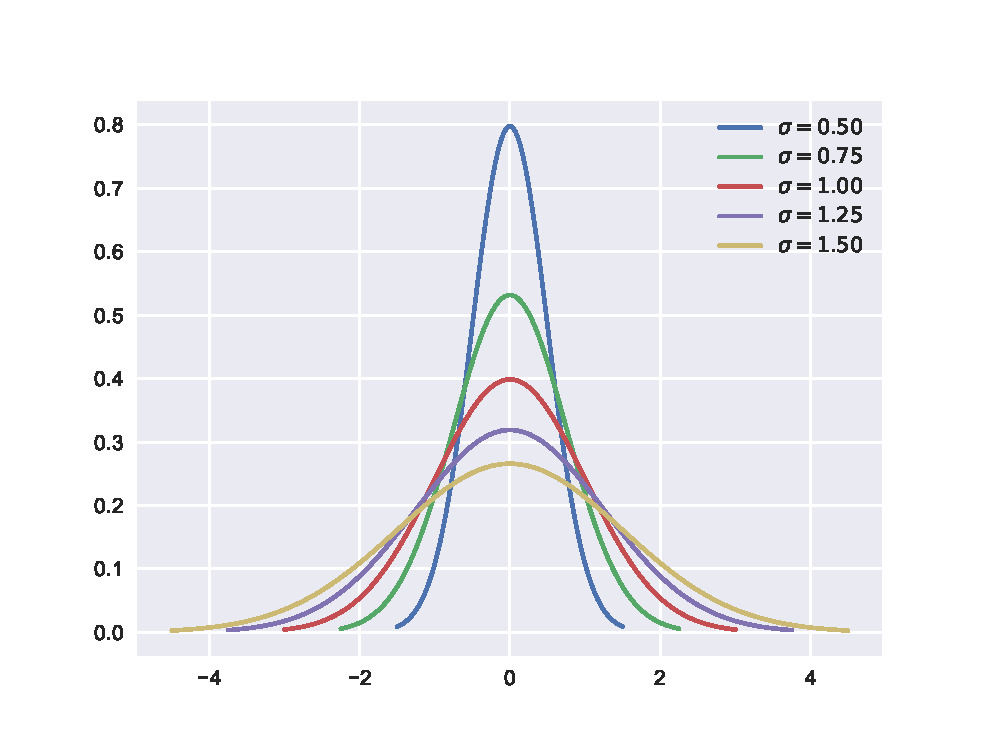
\includegraphics[width=0.7\textwidth]{images/normalPlot.eps}}
\caption{Normal distribution with different standard deviations}
\label{fig:normal_plot}
\end{figure}



In this chapter we looked at three different kinds of algorithms each designed to solve the RL problem.
We presented many extensions to each of these algorithms and in the end presented a new approach also.
In the next chapter we will look at how all of these algorithms performed on different tasks to eventually solve the snake simulation.


		\chapter{Evaluation}
\label{section:results}

In the following section we will compare the different algorithms in three different experiments.
Each experiment will be described, the results will be presented and interpreted.
First we will look at two fairly simple environments, one that acts in discrete space and one that acts in continuous space.
These environments are used to better understand the algorithms used in this thesis.
In the end we will look at the actual problem of this paper, the application of these algorithms on the snake-like environment.
Note that all graphs in this section are smoothed by a Savitzky-Golay-Filter for better display.

\section{CartPole-v0}

The first environment we chose was the \emph{CartPole-v0} environment.
Table \ref{tb:cartpole_specs} shows the specification of this environment.

\begin{table}[H]
  \centering
  \begin{tabular}{| c | c |}
      \hline
      Observation space & Continuous\\
      \hline
      Num Observations & $4$\\
      \hline
      Action Space & Discrete\\
      \hline
      Num Actions & $2$\\
      \hline
  \end{tabular}
\caption{Specification of the CartPole-v0 environment}
\label{tb:cartpole_specs}
\end{table}

\subsection{Goals}

The objective of the CartPole-v0 is to balance a pole on a cart that can move left or right.
This is a discrete problem because we can either push left with full force or right with full force.
In the beginning of each episode the cart is spawned in the center of the screen and the pole is initialized with a small random angle..
The agent receives $1$ reward for every time step it keeps the pole balanced.
An episode terminates if the pole falls too far to one side or the cart moves too far to one side.
It is solved when obtaining an average return of $195$ over $100$ consecutive episodes.
We chose this environment to start off with because it is a discrete environment with only two actions and only four observations.
It is considered a very easy to solve environment.
DQN is known to act better in discrete action spaces which makes this environment a perfect fit.
This was the first environment we trained our first algorithm on and was more of a testing stage for later problems to come.

\subsection{Realization}

We'll run our algorithms for 1000 episodes which corresponds to roughly 1 hour of training.
The data will be collected by simply cumulating all rewards we observed in one episode.
At first we will run the basic DQN and then add all extensions to it and run it again.
Table \ref{tb:dqn_params} shows the hyperparameters we'll use for the DQN with and without extensions.

\begin{table}[H]
  \centering
  \begin{tabular}{| c | c |}
      \hline
      Hyperparameter & Value\\ \hline
      Layer 1 size & $20$\\
      Layer 2 size & $20$\\
      Batch size & $20$\\
      Target Update Freq. & $50$\\
      $\alpha$ & $0.00025$\\
      $\gamma$ & $0.9$\\
      $\epsilon$ & $0.1$\\
      \hline
  \end{tabular}
\caption{Hyperparameter configuration for Dueling DQN with PER}
\label{tb:dqn_params}
\end{table}


\subsection{Results}

\begin{figure}[H]
\centerline{
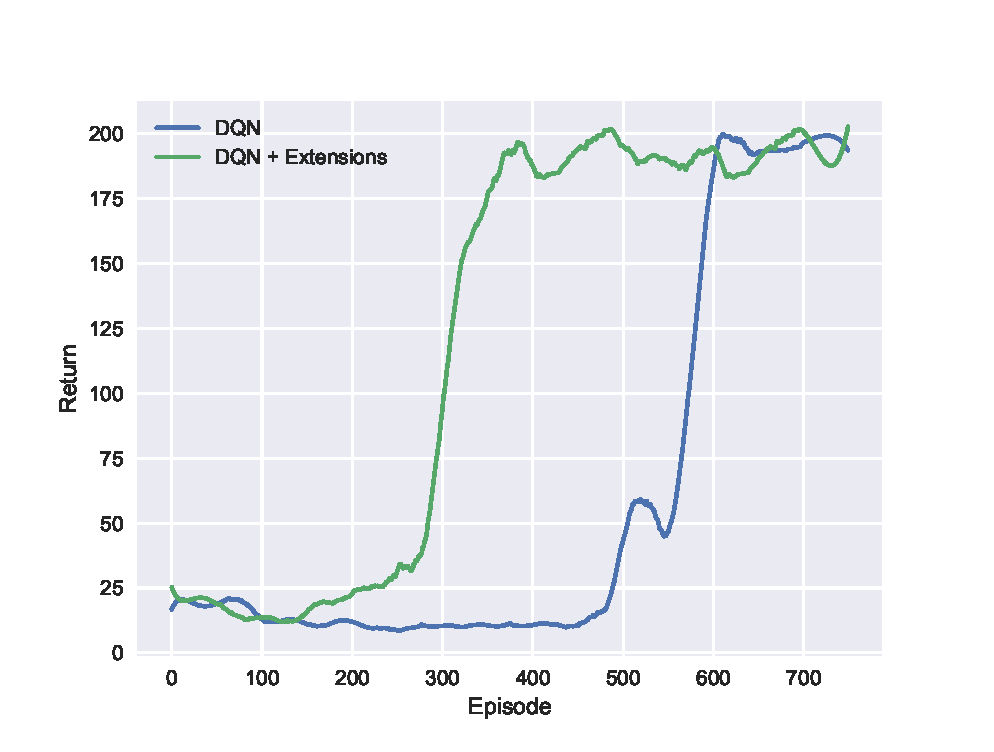
\includegraphics[width=0.7\textwidth]{images/dqn_compare_cartpole.eps}}
\caption{Comparison of the algorithms on the CartPole-v0 environment}
\label{fig:cartpole_compare}
\end{figure}

Figure \ref{fig:cartpole_compare} shows the results for this environment.
As one can see the steep learning curve appears around 200 episodes earlier when extensions are applied.
Because all hyperparameters were the same in both runs it is clear that the extensions actually have a positive impact on the learning curve.
In our experiment the DQN with extensions solved the environment after around 400 episodes while the basic DQN took around 700 episodes to solve it.
This means that the extensions required around 40\% less training data to solve the environment.


\section{Pendulum-v0}

Next we move from the discrete action-space of the CartPole-v0 environment to the continuous
action-space of the Pendulum-v0 environment.
Table \ref{tb:pendulum_specs} shows the specifications of this environment.

\begin{table}[H]
  \centering
  \begin{tabular}{| c | c |}
      \hline
      Observation space & Continuous\\
      \hline
      Num Observations & $3$\\
      \hline
      Action Space & Continuous\\
      \hline
      Action Dimensions & $1$\\
      \hline
  \end{tabular}
\caption{Specification of the Pendulum-v0 environment}
\label{tb:pendulum_specs}
\end{table}

\subsection{Goals}

The goal of this environment is to swing up a pendulum and then balance it.
The agent can achieve this by applying a force to the pendulum pushing it either to the left or to the right.
In the beginning of each episode the pendulum is initialized in a random position.
Each episode terminates exactly after $200$ timesteps.
The agent receives a small negative reward in each timestep corresponding to the degree it is off from balancing it straight up.
E.g. if it hangs loosely downwards it would be 180° off which is the worst possible position.
With this environment we want to make a smooth transition from the easy discrete environment of the CartPole-v0 to our continuous snake-like environment.
The Pendulum-v0 is still a considerably simple to solve environment but as already mentioned acts in a continuous space.
We want to see from this experiment which algorithms are worth trying on the snake-like environment.

\subsection{Realization}

In this experiment we will use the same hyperparameters for DQN as before.
We will only run the version with extensions applied.
Again the data will be collected by simply cumulating all rewards we observe in one episode.
All algorithms will run for just 200 episodes.
Table \ref{tb:ddpg_params} shows the hyperparameters we'll use for all our DDPG experiments.
We will look at how DQN performs on this task and then compare it to DDPG with and without parameter noise applied.

\begin{table}[H]
  \centering
  \begin{tabular}{| c | c |}
      \hline
      Hyperparameter & Value\\ \hline
      Layer 1 size & $200$\\
      Layer 2 size & $200$\\
      Batch size & $32$\\
      Learning Rate Actor & $0.0001$\\
      Learning Rate Critic & $0.001$\\
      Replay Memory Size & $1000000$\\
      $\tau$ & $0.001$\\
      \hline
  \end{tabular}
\caption{Hyperparameter configuration for DDPG}
\label{tb:ddpg_params}
\end{table}

\subsection{Results}

\begin{figure}[H]
\centerline{
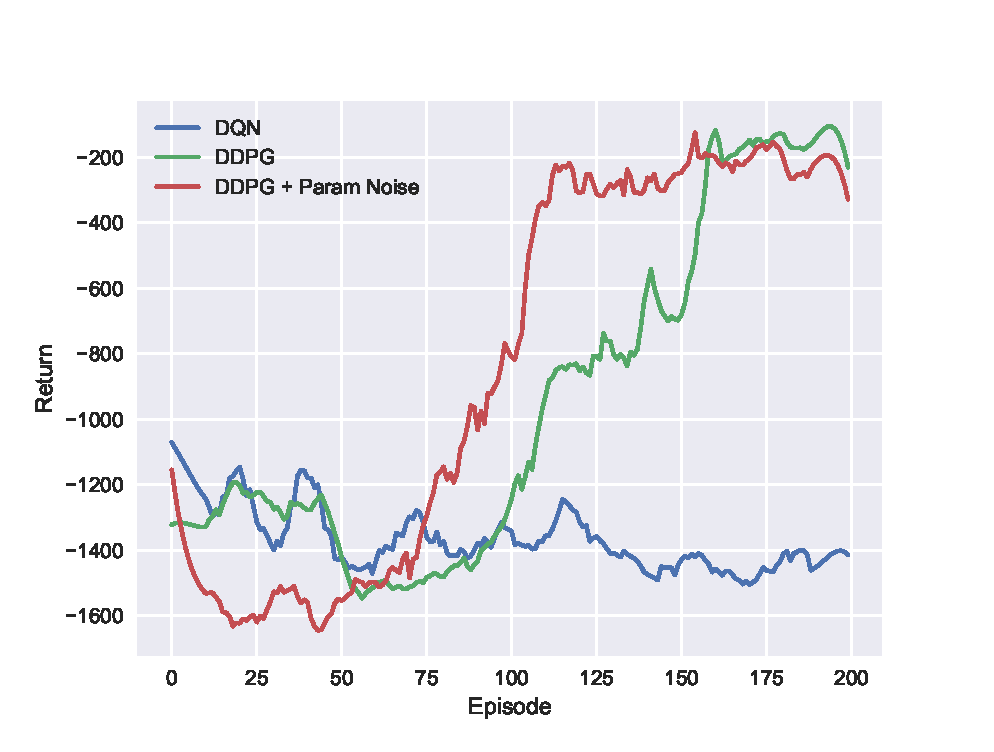
\includegraphics[width=0.7\textwidth]{images/pendulum_compare.eps}}
\caption{Comparison of the algorithms on the Pendulum-v0 environment}
\label{fig:pendulum_compare}
\end{figure}

Figure \ref{fig:pendulum_compare} shows the results for all three runs in this environment.
Unfortunately DQN failed to learn a useful policy on this task.
DDPG on the other hand learned a good policy after only 200 episodes of training and adding parameter
noise to it returned even better results. Because the DQN failed on this task
already we decided not to try it on the snake as the Curse of Dimensionality [1] makes it
an even harder problem for DQN.

\section{Swimmer-v1}

After successfully solving the Pendulum-v0 we now move on to the Swimmer-v1 environment.
This environment is the main environment of this thesis because it represents a snake-like robot very closely.
It has two joints that can be moved in any direction to produce movement. Table \ref{tb:swimmer_specs} shows the specifications for this environment.

\begin{table}[H]
  \centering
  \begin{tabular}{| c | c |}
      \hline
      Observation space & Continuous\\
      \hline
      Num Observations & $8$\\
      \hline
      Action Space & Continuous\\
      \hline
      Action Dimensions & $2$\\
      \hline
  \end{tabular}
\caption{Specification of the Swimmer-v1 environment}
\label{tb:swimmer_specs}
\end{table}


\subsection{Goals}

The goal is to move the robot as far to the right as possible. The agent receives a small positive or negative reward in each timestep according to a reward function that takes into account the position of the snake relative to the starting point and the smoothness of the movement.
With this experiment we want to see which algorithm produces the best results on a snake-like robot.
We also want to look at our new way of introducing noise to the PPO.

\subsection{Realization}

We'll again use the same hyperparameters for DDPG as before and again compare DDPG with and without action noise.
At first we will only look at PPO without additional noise factors and later compare those results separately.
We will run all our experiments on this environment for $1500$ episodes.
Note that it makes a significant difference in computational time whether to use DDPG or PPO.
While DDPG takes around 10 seconds per episode, PPO takes nearly no time for a single episode and only takes around a few seconds of training time after one trajectory.
Table \ref{tb:ppo_params} shows the hyperparameters used for all PPO experiments.
\begin{table}[H]
  \centering
  \begin{tabular}{| c | c |}
      \hline
      Hyperparameter & Value\\ \hline
      Layer 1 size & $100$\\
      Layer 2 size & $100$\\
      Trajectory size & $5$\\
      Learning Rate Actor & $0.00025$\\
      Learning Rate Critic & $0.0025$\\
      $\gamma$ & $1$\\
      $\lambda$ & $0.98$\\
      $\epsilon$ & $0.2$\\
      \hline
  \end{tabular}
\caption{Hyperparameter configuration for PPO}
\label{tb:ppo_params}
\end{table}

\newpage

\subsection{Results}

\begin{figure}[H]
\centerline{
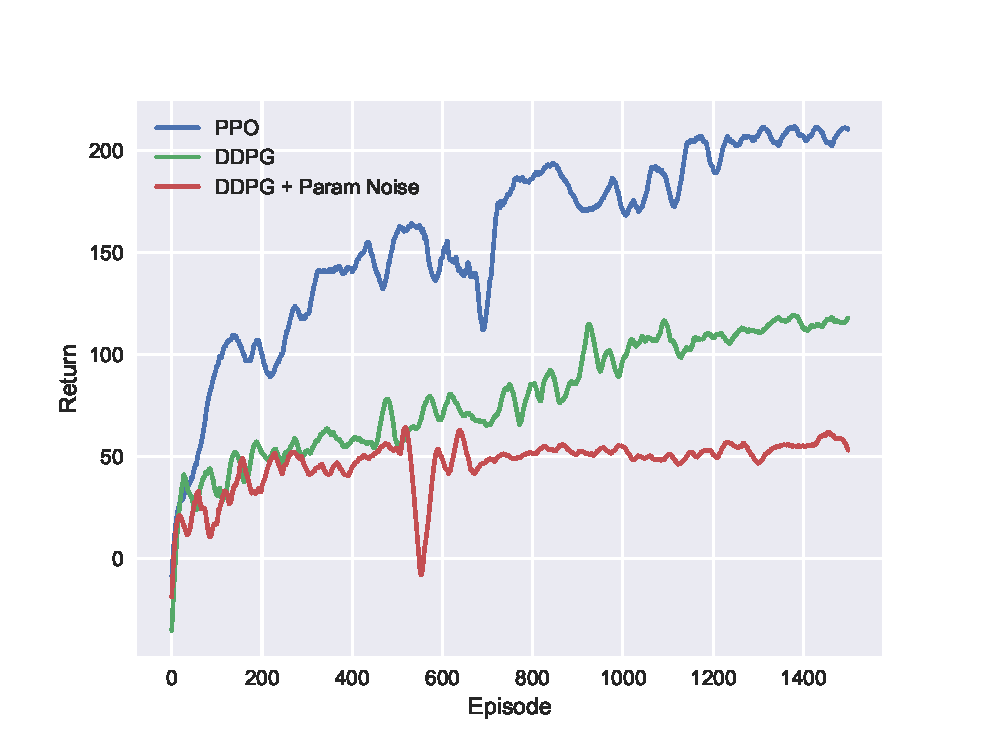
\includegraphics[width=0.7\textwidth]{images/snake_compare.eps}}
\caption{Comparison of the algorithms on the Swimmer-v1 environment}
\label{fig:snake_compare}
\end{figure}

Figure \ref{fig:snake_compare} shows all results of our different algorithms.
As one can see the DDPG gets stuck in a local maximum after some time at around 120. This is a known problem
for DDPG algorithms when dealing with more complex problems. Although the variance
of different runs is pretty small for the DDPG. This means that on every run it settles at a
score of around 120 after 1000 to 1500 episodes. For some reason adding parameter noise
to it now makes the performance way worse. We were not able to reproduce the desired
results of the original paper for this environment.


PPO is better and settles at a score of around 200 after 1500 episodes. The problem here
is that the variance for PPO is very high. In these graphs we only include the best runs of
all algorithms.

\newpage

\begin{figure}[H]
\centerline{
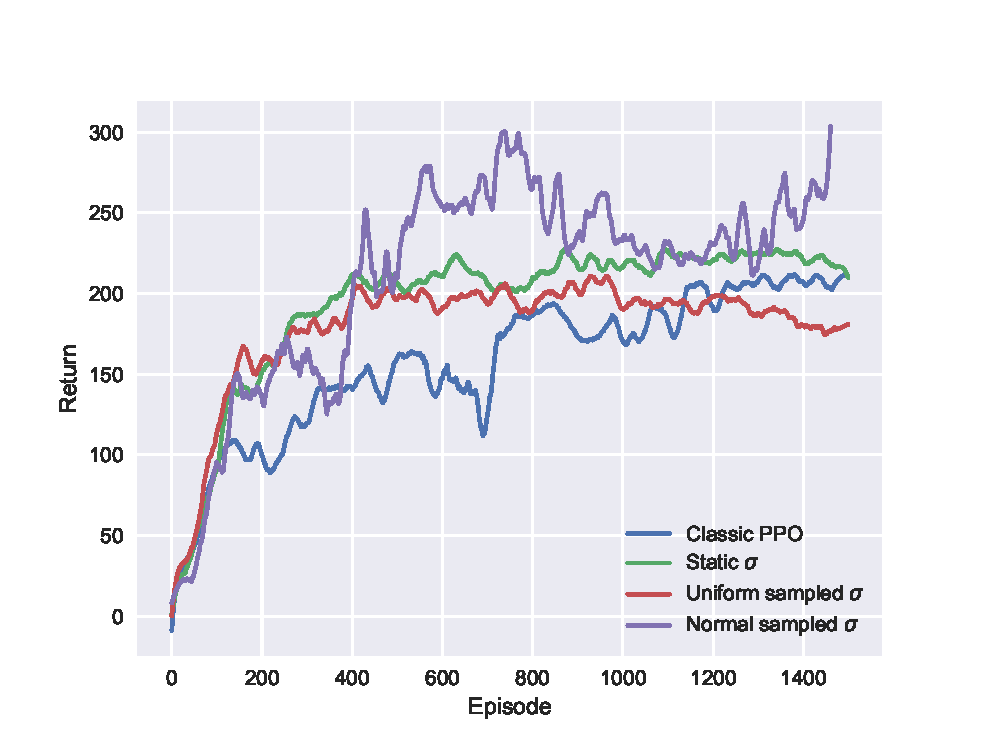
\includegraphics[width=0.7\textwidth]{images/ppo_compare_noise.eps}}
\caption{Comparison of different noise factors}
\label{fig:ppo_noise_compare}
\end{figure}

Lastly we compared our different approaches to add noise to the PPO.
Figure \ref{fig:ppo_noise_compare} shows the best runs for all algorithms.
The graph for classic PPO is the same as in Figure \ref{fig:snake_compare} and is only added to give a reference to the other graphs.
Keeping the standard deviation static seems to be a little more stable and settles after only 400 episodes at a score of 200.
Sampling from a uniform distribution before every trajectory makes no difference compared to the classic PPO.
By sampling the standard deviation from a normal distribution though we achieved a score of over 300 after 1500 episodes.
This is a significant improvement towards the classic PPO algorithm and all of our other approaches.
The high achievement in the beginning of the learning process can probably be linked to better exploration.


In this chapter we set up three different experiments for all the algorithms.
We started off by looking at fairly simple problems at first before moving on to the more complex problem of the snake-like robot.
In the end we also looked at our new way of introducing noise to PPO and compared different ways to do so.
In the next section we will conclude the findings of this thesis and present future work.


		\chapter{Conclusions and Future Work}
\label{section:conclusion}

In this thesis we looked at different algorithms to solve the \emph{Swimmer-v1} environment.
We observed that DQN is not suited to solve tasks in continuous action space, at least not by simply discretizing the action space.
We also found that the biggest problem of DDPG is that it settles in local maximums rather than finding a global one.
PPO achieved the best results of all the algorithms tried in this thesis.
From our results it looks like PPO or at least policy gradient based methods seem to be the best way at the moment to solve high dimensional tasks.


Our newly introduced way to increase exploration in PPO actually made a significant improvement in our experiments.
But there are still many things to improve in order to get a good and stable algorithm.
The \emph{Swimmer-v1} environment is supposed to be completely solved when getting an average return of 360 over 100 consecutive trials.
Unfortunately none of the algorithms in this thesis achieved this but our new approach got the closest with an average return of 300.

Enhancements that could further increase performance:

\begin{itemize}
  \item The biggest problem we encountered during this thesis was the high variance of the PPO.
  In some runs it achieved results of well over 200 while in others it oscillated between 150 and 200.
  Future work could try to lower this variance in order to get a more stable algorithm.
  \item PPO is a stochastic algorithm. But in an environment like this it might be better to use a deterministic approach.
  Even though DDPG did not achieve high returns in this thesis it might be adopted in the future to make use of the good parts of PPO while still being deterministic.
  \item Varying the standard deviation yielded good results even if the approach is still very basic.
  One might be able to adopt the rate of exploration in a more clever way by maybe using something like a trust-region where exploration is slowed down if the network changes too fast and increased if it changes too slow.
  \item Instead of changing the standard deviation it might be better to change the whole distribution, morphing it from a tight normal distribution towards a uniform distribution according to the wanted rate of exploration.
\end{itemize}


    \appendix{}

    \listoffigures
    % \listoftables
    % \listofalgorithms

    \clearemptydoublepage

	  \bibliography{bibliography/literature}

    \clearemptydoublepage

    \addchap{Glossary}
\bgroup
\def\arraystretch{1.5}
\begin{longtable}{p{0.25\textwidth} p{0.705\textwidth}}
  RL & Reinforcement Learning \\
  AI & Artificial Intelligence \\
  ML & Machine Learning\\
  NN & Neural Network\\
  DNN & Deep Neural Network\\
  MDP & Markov Decision Process\\
  TD & Temporal Difference\\
  MC & Monte Carlo\\
  SARSA & State–action–reward–state–action\\
  MLP & Multi-Layer-Perceptron\\
  CNN & Convolutional Neural Network\\
  MSE & Mean Squared Error\\
  CUDA & Compute Unified Device Architecture\\
  GPU & Graphical Processing Units\\
  CPU & Central Processing Unit\\
  TF & Tensorflow\\
  VREP & Virtual Robot Experimentation Environment\\
  ROS & Robot Operating System\\
  API & Application Programming Interface\\
  MuJoCo & Multi-Joint dynamics with Contact\\
  DQN & Deep-Q-Network\\
  ERM & Experience Replay Memory\\
  PER & Prioritized Experience Replay\\
  DDPG & Depp Deterministic Policy Gradient\\
  PPO & Proximal Policy Optimization\\
  TRPO & Trust Region Policy Optimization\\
  GAE & General Advantage Estimation\\
\end{longtable}
\egroup

    \addchap{Notation}
\bgroup
\def\arraystretch{1.5}%  1 is the default, change whatever you need
\begin{longtable}{p{0.25\textwidth} p{0.705\textwidth}}
  $t \in \mathbb{N}$ & Timestep \\
  $S$ & Set of states\\
  $s_t \in S$ & State in timestep $t$\\
  $d_a \in \mathbb{N}$ & Action space dimension\\
  $a_t \in \mathbb{R}^{d_a}$ & Continuous action in timestep $t$\\
  $a_t \in \mathbb{N}^{d_a}$ & Discrete action in timestep $t$\\
  $r_t \in \mathbb{R}$ & Reward in timestep $t$\\
  $\mathbb{P}[S_t] \in \mathbb{R}$ & Probability of observing state $S_t$\\
  $\mathbb{P}[S_{t+1} | S_t] \in \mathbb{R}$ & Probability of observing state $S_{t+1}$ in state $S_t$\\
  $\gamma \in [0,1]$ & Discount factor\\
  $G_t \in \mathbb{R}$ & Discounted sum of reward also called return\\
  $v(s)$ & Value of state $s$\\
  $\pi(a|s)$ & Probability of choosing action $a$ in state $s$ also called policy\\
  $v_\pi(s)$ & State-value function following policy $\pi$\\
  $q_\pi(s,a)$ & Action-value function following policy $\pi$\\
  $\pi_*(a|s)$ & Optimal Policy for a given MDP\\
  $v_*(s)$ & Value function of the optimal policy $\pi_*$\\
  $q_*(s,a)$ & Action-value function of the optimal policy $\pi_*$\\
  $\epsilon \in [0,1]$ & Amount of random actions\\
  $N$ & Set of neurons in a neural network\\
  $V$ & Set of connections between two neurons\\
  $w_{(i,j)} \in \mathbb{R}$ & weight of the connection between neuron $n_i$ and $n_j$\\
  $\alpha \in [0,1]$ & Learning Rate\\
  $\Delta w_{(i,j)} \in \mathbb{R}$ & Change of weight $w_{(i,j)}$\\
  $\theta \in \mathbb{R}^{N \times M}$ & Trainable parameters of a neural network\\
  $\hat{q}(s,a, \theta)$ & Action-value function approximation with parameters $\theta$\\
  $\pi_\theta(a|s)$ & Policy approximation with parameters $\theta$\\
  $J(\theta)$ & Objective function approximation with parameters $\theta$\\
  $\nabla_{\theta}J(\theta)$ & Gradient of $J(\theta)$ w.r.t. $\theta$\\
  $\alpha, \beta \in [0,1]$ & Exponents of prioritized replay memory\\
  $A(s,a)$ & Advantage function\\
  $\tau \in [0,1]$ & Update rate for soft target update\\
  $\mathcal{N}_t$ & Random process in timestep $t$\\
  $\widetilde \theta$ & Network parameters with applied parameter noise\\
  $\sigma$ & Standard deviation of a probability distribution\\
  $r_t(\theta)$ & Probability ratio in timestep $t$ with parameters $\theta$\\
  $L(\theta)$ & Surrogate objective function\\
  $\hat{A}_t^{GAE(\gamma,\lambda)}$ & General Advantage estimate using parameters $\gamma,\lambda$\\


\end{longtable}
\egroup



\end{document}
